%\documentclass{../_combined/fcg-book}
\chapter{The Guessing Game} \label{chap:6}

The problem how a physically embodied situated agent
might refer to objects using language is extraordinarily 
difficult. If we then further want to find out how 
a group of such agents might autonomously bootstrap
a language system, the task seems almost unsurmountable. 
That is why I proposed earlier on to start by dividing
this task into its three main subtasks along the lines
of the semiotic square (\figref{square6}).
The previous chapters each focused on one of these tasks. 
Chapter~5 has introduced 
perceptual mechanisms to process the raw image, segment
the scene, derive characteristics about each 
segment, and give feedback by pointing to the referent. 
Chapter~4 studied categorisation mechanisms
needed for conceptualising a scene and thus for 
generating the possible meanings of a verbal
communication. Chapter 5 looked at how agents can 
lexicalise meanings and build up a sufficiently shared
lexicon to engage in verbal interactions. 

Given that we now have reasonable solutions for these
basic processes, at least for its most simple instantiations, 
we can now start to put the pieces together and thus
study the complete guessing game. I will 
proceed in two steps. First I will but the lexical 
layer and the conceptualisation layer together in 
this chapter, and then I will ground the whole system 
by coupling the conceptualisation layer to the 
perceptual layer in Chapter 7. 

Another technique I proposed earlier on 
for handling the enormous challenges addressed in 
this book, is to scale up 
gradually. I will follow this strategy as well. In this
chapter, I will assume that the referent and the 
perceived image are the same. This implies that we 
are really dealing with semiotic triangles as 
opposed to semiotic squares (\figref{square6}). 
I will start simulations with only 2 agents and then 
scale up to a larger number. This increases the degree
of synonymy in the lexicon. I will furthermore
start by letting the agents 
consider only the most salient channel, so that 
they much more easily guess the same category for the 
same scene. Then I will scale this up so that 
the agents now consider more sensory channels and hence
more categories. This increases the degree of 
ambiguity in the lexicon. Both synonymy and ambiguity 
are sources of incoherence and we will have to make
sure that agents still manage to be successful 
despite of these. 

This chapter shows that agents still manage to 
bootstrap a shared lexicon due to carefully established
feedback couplings between the different processing
layers introduced in the previous chapters. 
The language game gives feedback to the lexical layer so 
that words become preferred that are understood by others.
The lexical layer gives feedback to the conceptual layer
so that categories become preferred that have been
successfully lexicalised. Each layer is a selectionist system
that generates possible ways to solve a subproblem, of which some 
are kept and others discarded based on feedback of their use.
I will examine in this chapter whether these
couplings indeed cause a coordination of the different internal
layers in a single agent and whether they lead to shared 
ontologies and lexicons. 

\section{Defining the Guessing Game}

The guessing game was already introduced in Chapter 2. Here is a first example game, game 500.\is{Guessing Game}
{\bfshape  a2} plays the role of speaker and {\bfshape  a1} the role of hearer. The game is about the scene in
\figref{rect1}. The topic is the rectangle labeled 1. The grayscale channel is the most 
salient channel. The different sensory values (after sensor-scaling)
for the segments in \figref{rect1} are shown in 
\tabref{tab:t-rect1}. The last line shows the saliency of 
the topic segment 1.  Clearly the grayscale channel is the most salient. 


\begin{table}
\begin{center}
\begin{tabular}{ l  l  l  l  l  l  l }
\lsptoprule
{\itshape obj} & HPOS & VPOS & HEIGHT & WIDTH & GRAY & AREA \\ \midrule
0 & 0.66 & 0.95 & 0.01 & 0.71 & 0.19 & 0.27\\ 
1 & 0.69 & 0.83 & 0.07 & 0.33 & 0.97 & 0.21\\ 
2 & 0.99 & 0.87 & 0.54 & 0.72 & 0.22 & 0.57\\ 
saliency & 0.03 & 0.05 & 0.07 & 0.39 & 0.75 & 0.06 \\ 
\lspbottomrule
\end{tabular}
\caption{\label{tab:t-rect1}Sensory data for the scene shown in \figref{rect1}.}
\end{center}
\end{table}
All rectangles are relatively close to each other and have more or less the 
same height and width. But the grayscale is clearly the more salient because rectangle-1 is 
much darker than the others. I assume that there are only two agents in the population and that they always use only 
the most salient to conceptualise the scene. 
The speaker and hearer have to traverse only 
two sides of the semiotic square (\figref{square6})
because we assume that perceived image and object being
referred to are identical for both agents. 


\begin{figure}[htbp]
  \centerline{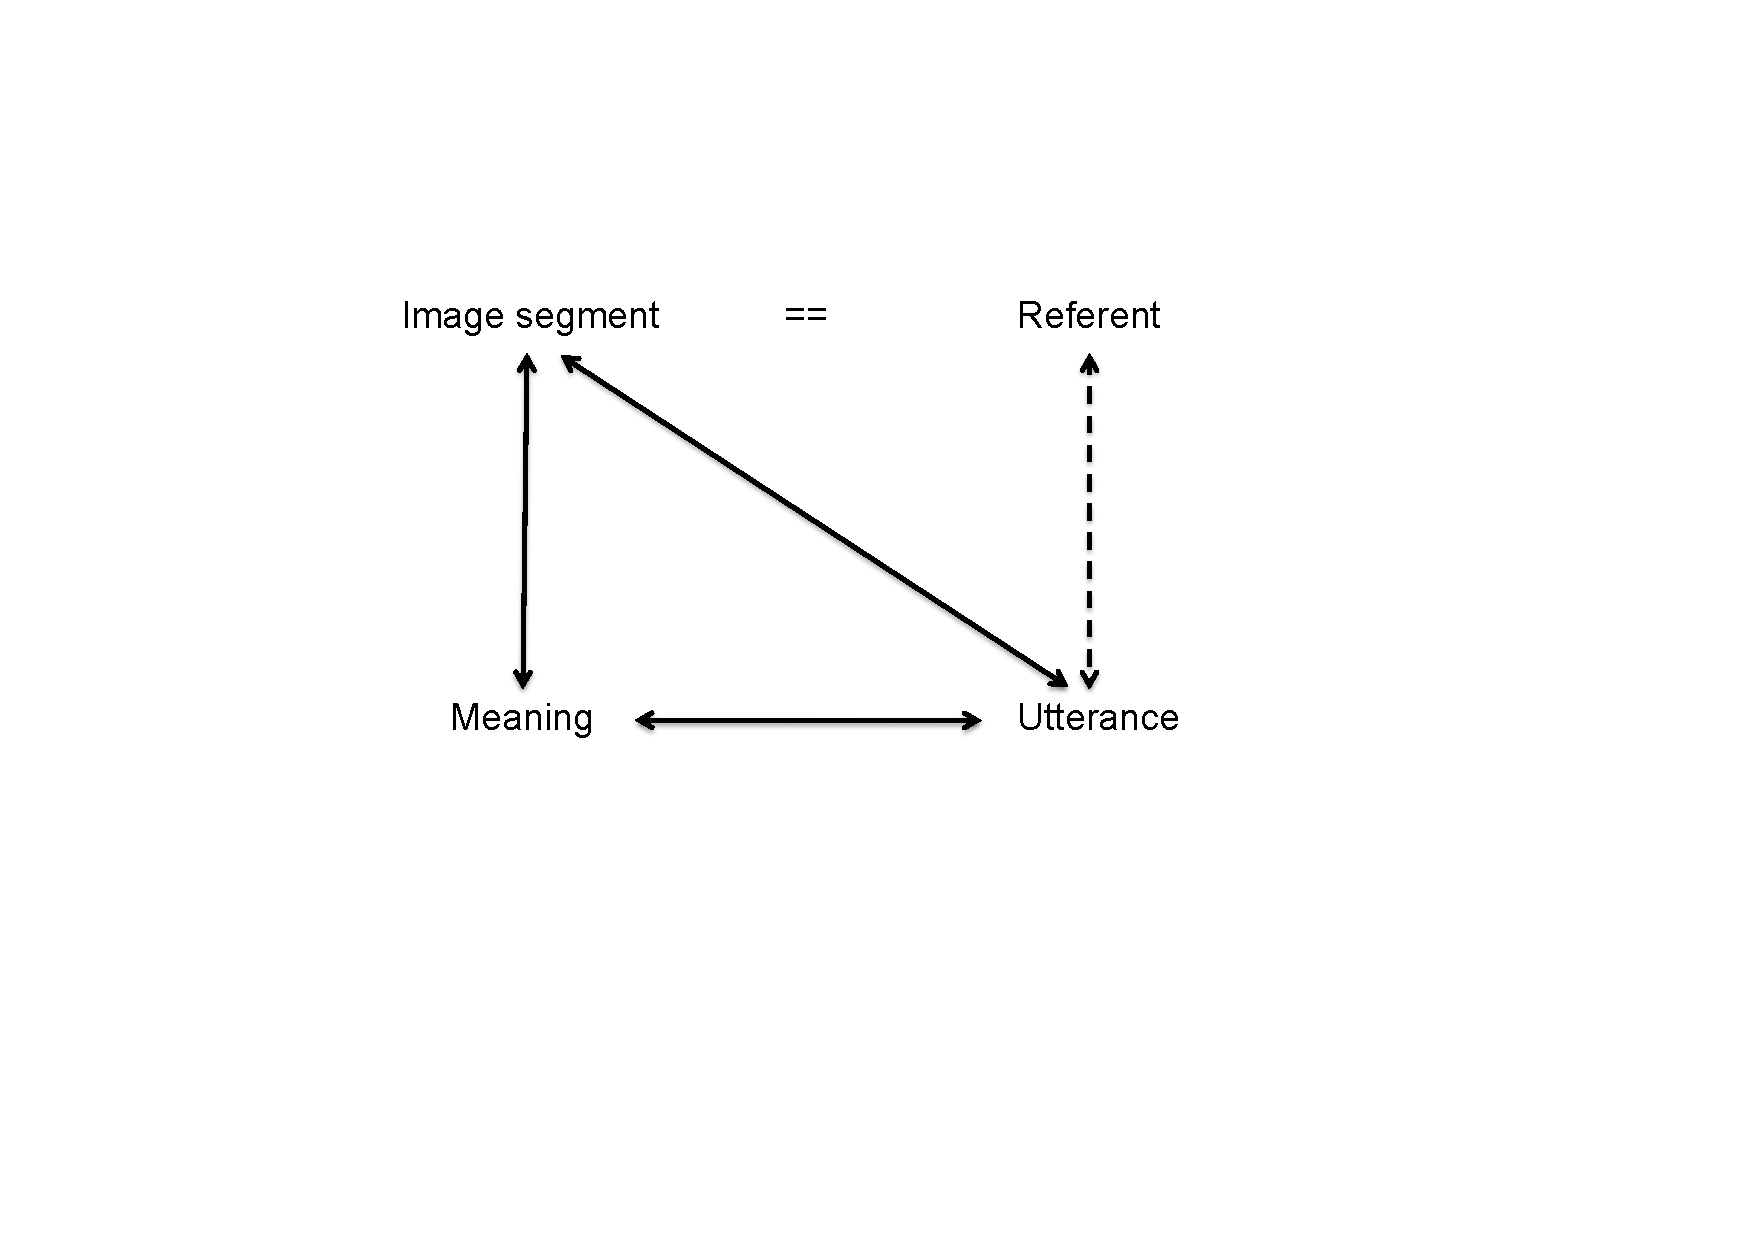
\includegraphics[width=.50\textwidth]{chap6/figs/square6.pdf}}
\caption{\label{square6}The semiotic square becomes
a triangle when the perceived image and the referent in the
real world are assumed to be identical.} 
\end{figure}

\subsection{Example of a coupled game}

The speaker first plays a Discrimination Game traversing the 
semantic side of the square going from the referent 
{\itshape rectangle-1} to a possible meaning [GRAY 0.5–1.0]. 
He then plays a Naming Game traversing the lexical side of 
of the square to find the word `pokuneso' for this chosen meaning. 
The hearer traverses the lexical side of the triangle in 
the other direction to interpret the word `pokuneso' as
{}[GRAY 0.5–1.0], and then identifies the referent by 
filtering the objects in the context with this meaning. 
Only rectangle-1 remains, so the game succeeds. 
The whole game is reported by the commentator as follows: 
\begin{verbatim}
Game 500
  a2 is the speaker. a1 is the hearer. 
  a2 segments the context into 3 objects: 
       rectangle-0 rectangle-1 rectangle-2
  a2 chooses rectangle-1 as the topic 
  a2 categorises the topic as [GRAY 0.5–1.0]
  a2 says: pokuneso
  a1 interprets pokuneso as [GRAY 0.5–1.0]
  a1 points to rectangle-1
  a2 signals OK 
\end{verbatim}
The game is perfectly successful because both 
agents associate the word `okuneso' with 
{}[GRAY 0.5–1.0] (dark) and they perceive the scene 
in the same way.


\begin{figure}[htbp]
  \centerline{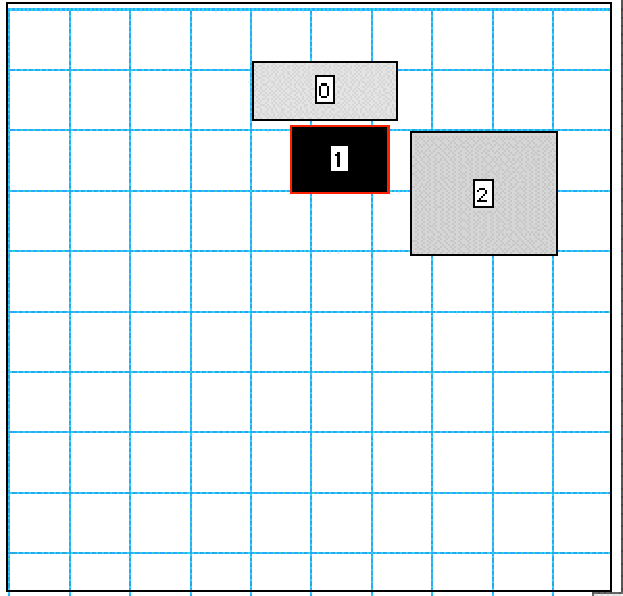
\includegraphics[width=.40\textwidth]{chap6/figs/recscene.pdf}}
\caption{\label{rect1}Example scene used
in game 500.}
\end{figure}



\begin{figure}[htbp]
  \centerline{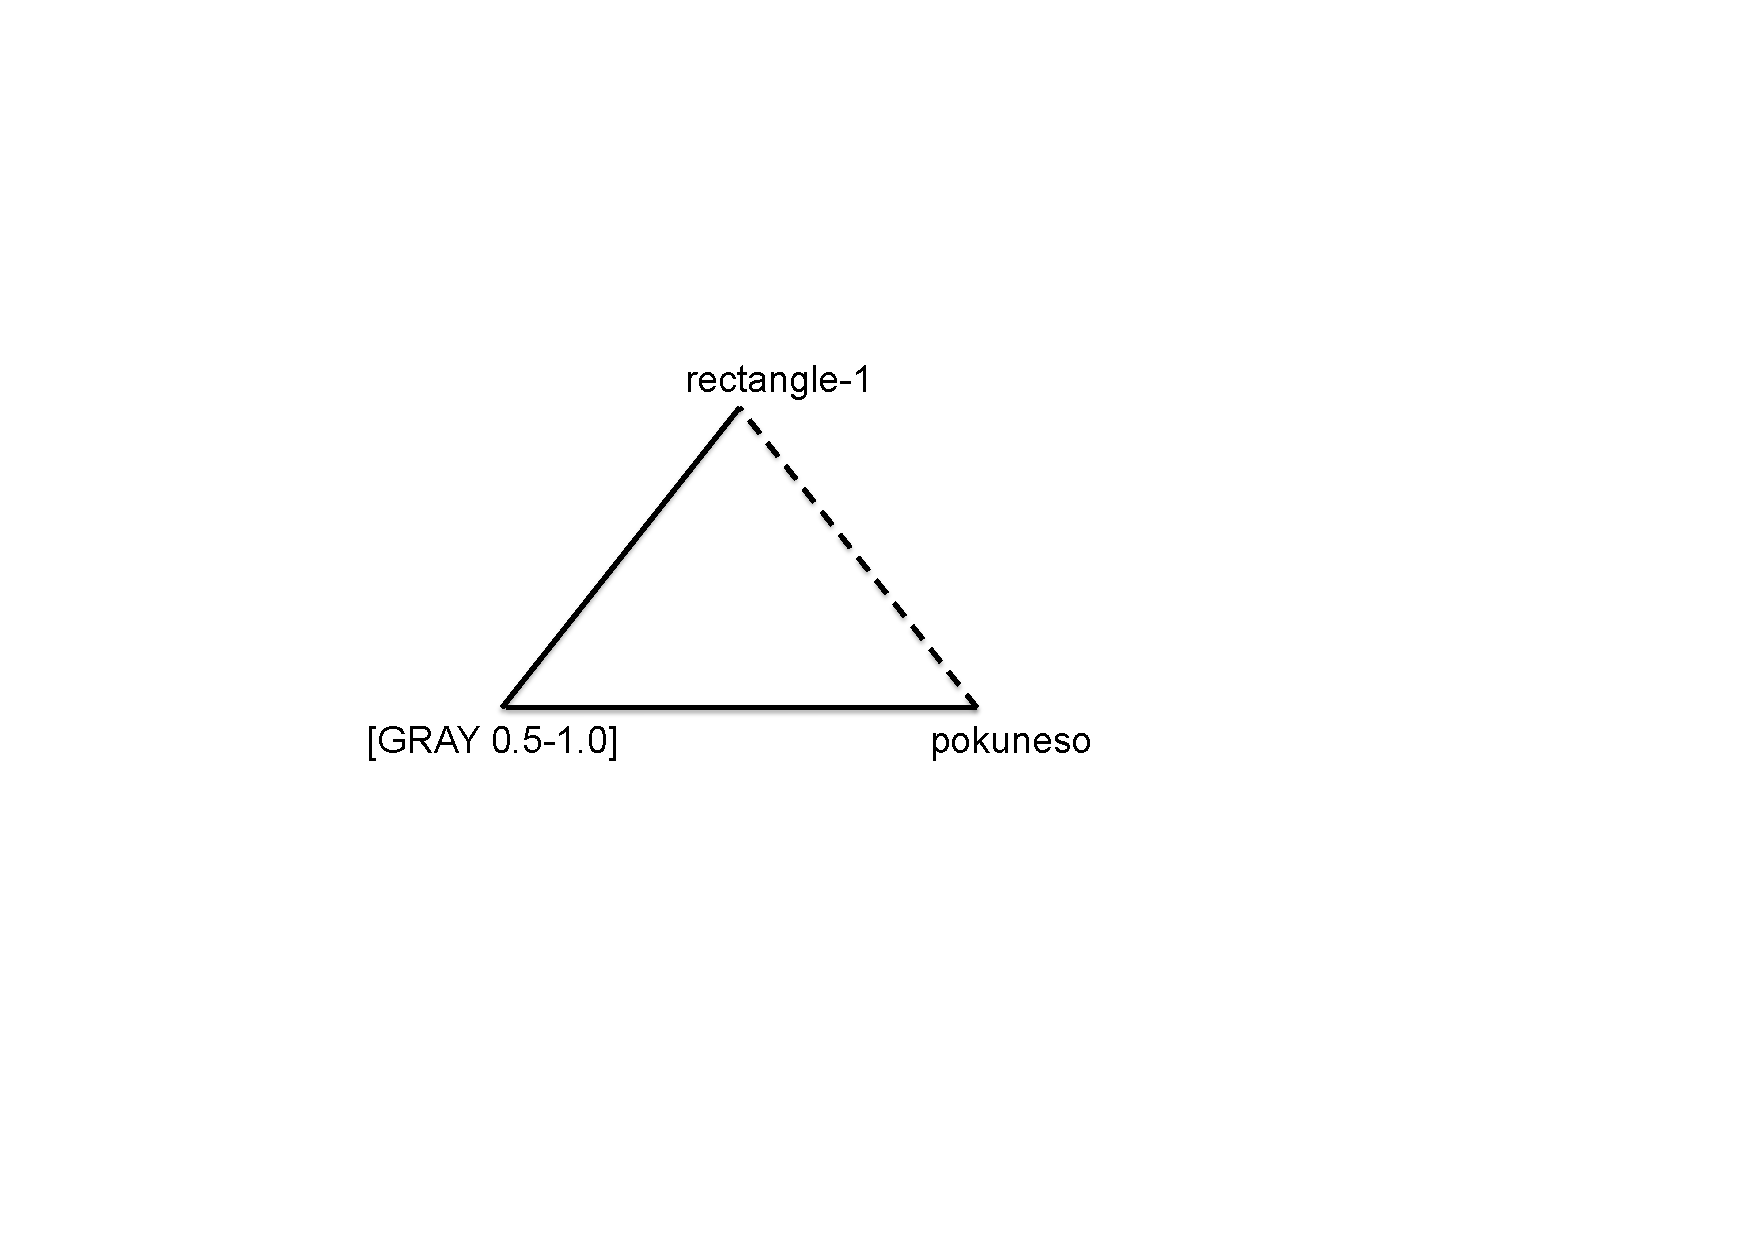
\includegraphics[width=.45\textwidth]{chap6/figs/triangle2.pdf}}
\caption{\label{triangle2}Semiotic triangle 
underlying game 500.}
\end{figure}

Before examining the architecture behind these
games in more detail, we can 
already see from \figref{gsuccess1} that
{\bfshape  a1} and {\bfshape  a2} clearly manage to build autonomously 
a communication system and its underlying ontology
from scratch by playing the 
guessing game. The communicative success 
moves up to reach almost 100 \% after a mere 500 games. 
Given that the environment keeps generating novel 
situations, there is always a chance that a 
scene occurs which requires new categories. So there 
is always a chance of failure, but it will 
further trigger expansion of the discrimination 
trees and of the lexicon. 


\begin{figure}[htbp]
  \centerline{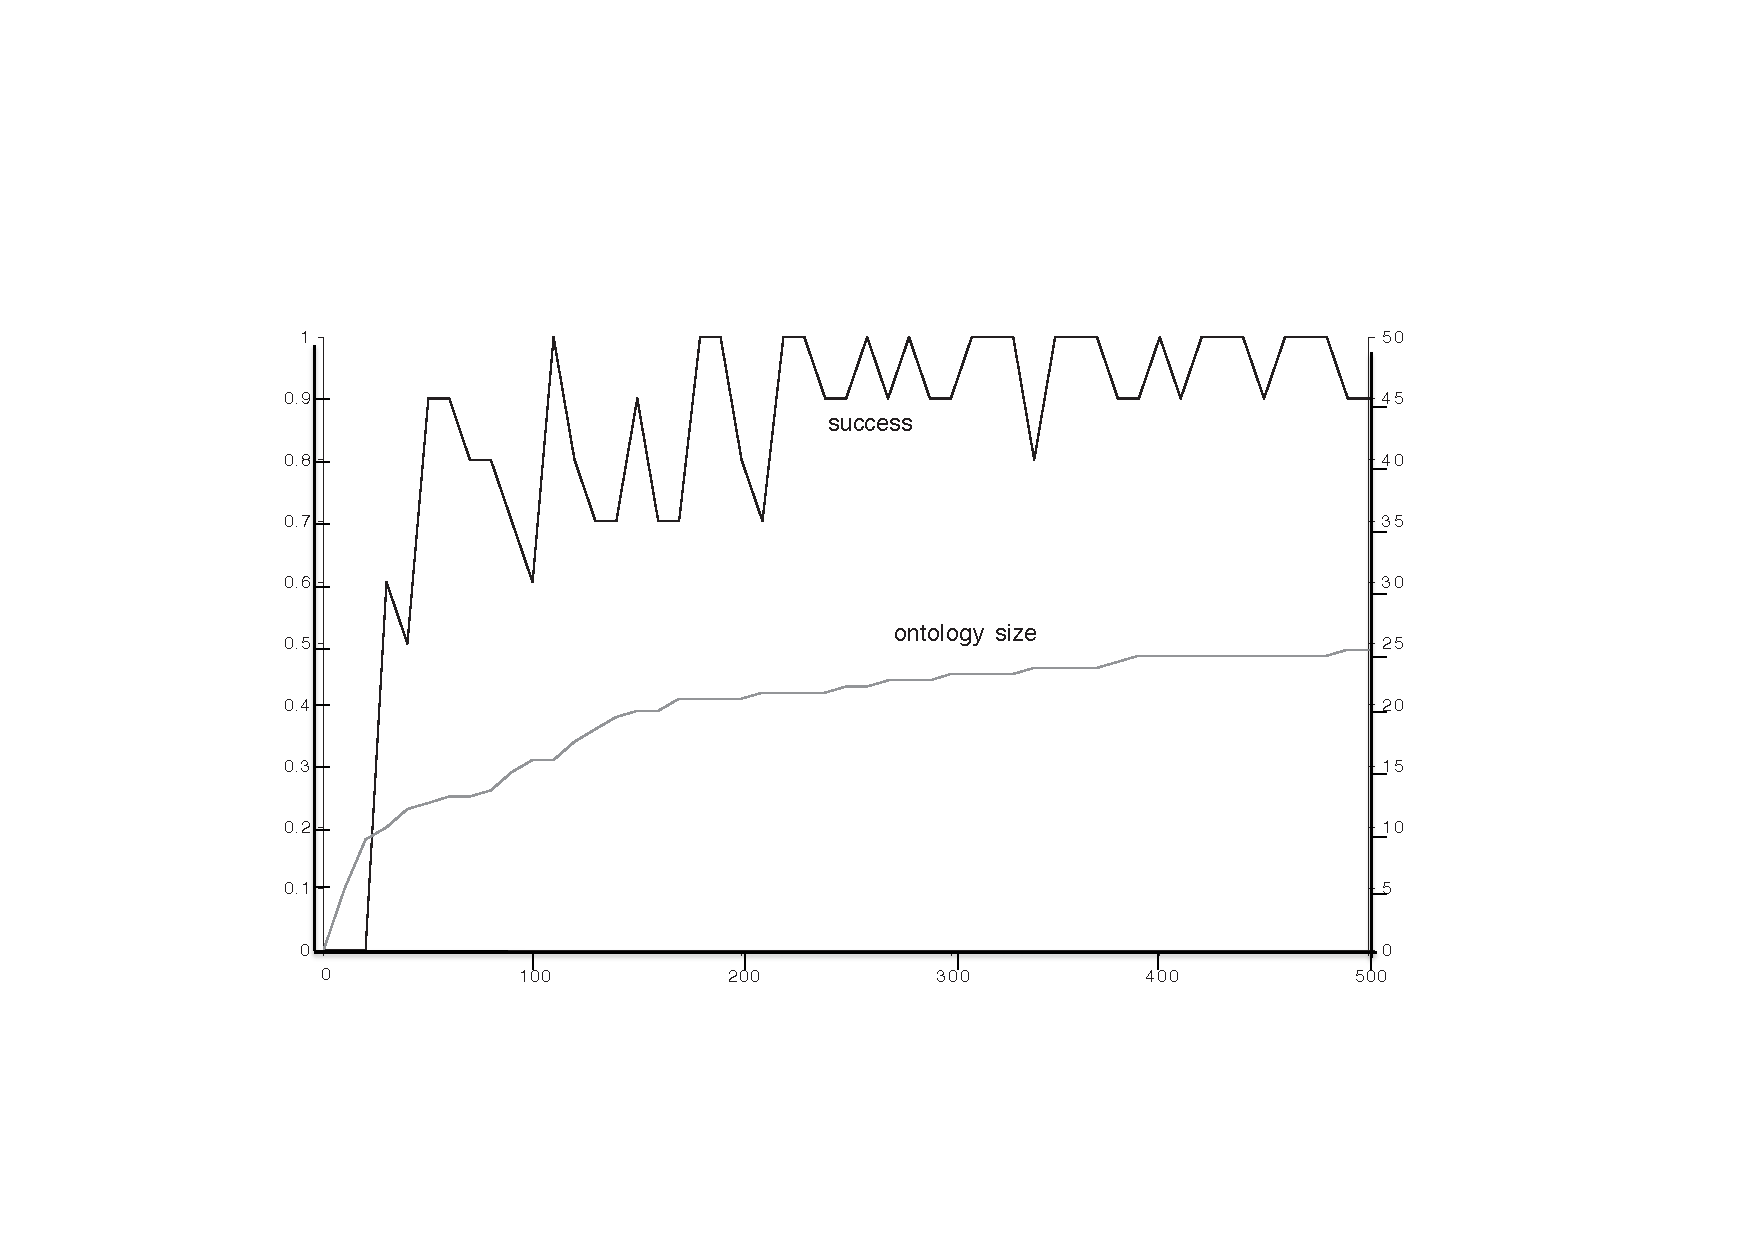
\includegraphics[width=\textwidth]{chap6/figs/gsucc1.pdf}}
\caption{\label{gsuccess1}Success 
(left y-axis) and average ontology size
(right y-axis) for two agents playing 500
guessing games.} 
\end{figure}
\figref{gsuccess1} also shows the average 
number of categories in each agent. There is a 
steep rise in the early phases, when no categories
exist, but then the creation of new categories levels 
off as discrimination mostly succeeds. When the 
environment becomes more complex, possibly exercising
additional sensory channels, the discrimination
trees would start to expand again, as we have seen 
in the previous chapter and then the lexicon 
would start to expand as well. Obviously the lexicon can only 
start to develop when there is an adequate ontology which 
explains some of the delay before the communicativesuccess curve starts to climb. 

\tabref{tab:lex100} displays the complete lexicon of the two agents after 100 games, 
together with the score for each assocation for 
{\bfshape  a1} and {\bfshape  a2}. Only associations where the 
score is above 0.0 for at least one agent are shown. 
A dash (-) indicates that the agent has not stored 
this association yet. 


\begin{table}
\begin{center}
\begin{tabular}{ l  l  l  l  l }
\lsptoprule
{\itshape Meaning}&{\itshape Word}&{\itshape Translation} & {\bfshape  a1}&{\bfshape  a2} \\ \midrule
{}[HPOS 0.0–0.5] & vapola&left&-&0.1\\ 
{}[HPOS 0.5–1.0]& gonapa&right &0.1&-\\ 
{}[HEIGHT 0.0–0.5]&suwaxugo&short &0.6&0.8\\ 
{}[HEIGHT 0.5–1.0]& kusone&tall &0.4&0.5\\ 
{}[WIDTH 0.0–0.5]&bepupepa&narrow &0.1&0.1\\ 
{}[WIDTH 0.0–0.25]&kutaki&very narrow &-&0.1\\ 
{}[WIDTH 0.5–1.0]& zikorika&wide &0.0&0.3\\ 
{}[GRAY 0.0–0.5]& fesasado&light &0.5&0.7\\ 
{}[GRAY 0.5–1.0]& pokuneso&dark &0.8&0.9\\ 
{}[AREA 0.5–1.0]& mafanoda&large &0.1&0.1\\ 
\lspbottomrule
\end{tabular}
\caption{\label{tab:lex100}. Complete lexicon of {\bfshape  a1} and {\bfshape  a2} after 100 games.}
\end{center}
\end{table}
We see that, at this point, the agents have lexicalised 
only the most general distinctions, such as dark (`pokuneso') 
versus light (`fesasado') or short (`suwaxugo') versus tall 
(`kusone'). Words for the grayscale and height dimensions
have the strongest scores, although this is purely accidental. 
When we would start another simulation from scratch,
we would end up with different words and perhaps 
other distinctions would be more successful. 

\tabref{tab:lex500a} is the complete lexicon after 500 games and \tabref{tab:lex500b} after 1000 games. 


\begin{table}
\begin{center}
\begin{tabular}{ l  l  l  l  l }
\lsptoprule
{\itshape Meaning}&{\itshape Word}&{\itshape Translation} & {\bfshape  a1}&{\bfshape  a2} \\ \midrule
{}[HPOS 0.0–0.5]&vapola&left &0.7&1.0\\ 
{}[HPOS 0.5–1.0]&gonapa&right &0.6&0.5\\ 
{}[VPOS 0.0–0.5]&rixuzime& up & 0.2&0.7\\ 
{}[VPOS 0.5–1.0]&gofugage& down &0.6&1.0\\ 
{}[HEIGHT 0.0–0.5]&suwaxugo&short & 1.0&1.0\\ 
{}[HEIGHT 0.0–0.25]&tawube&very short & 0.4&0.5\\ 
{}[HEIGHT 0.25–0.5]&narofi&medium short&0.1&0.4\\ 
{}[HEIGHT 0.5–1.0]&kusone&tall&1.0&1.0\\ 
{}[HEIGHT 0.5–0.75]&wuruzo&medium tall&0.3&0.6\\ 
{}[HEIGHT 0.75–1.0]&bowaluro&very tall&0.6&0.2\\ 
\lspbottomrule
\end{tabular}
\caption{\label{tab:lex500a}Lexicon of {\bfshape  a1} and {\bfshape  a2} after 500 games.}
\end{center}
\end{table}



\begin{table}
\begin{center}
\begin{tabular}{ l  l  l  l  l }
\lsptoprule
{}[WIDTH 0.0–0.5]&bepupepa&narrow & 1.0&1.0\\ 
{}[WIDTH 0.0–0.25]&kutaki&very narrow & 0.1&0.5\\ 
{}[WIDTH 0.25–0.5]&wukogo&medium narrow & 0.2&-\\ 
{}[WIDTH 0.5–1.0]&zikorika&wide & 1.0&1.0\\ 
{}[WIDTH 0.5–0.75]&mitula&medium wide &0.1&-\\ 
{}[WIDTH 0.75–1.0]&wupixo&very wide & -&0.2\\ 
{}[GRAY 0.0–0.5]&fesasado&light & 1.0&1.0\\ 
{}[GRAY 0.0–0.25]&sanize&very light & -&0.1\\ 
{}[GRAY 0.5–1.0]&pokuneso&dark &0.9&1.0\\ 
{}[GRAY 0.5–0.75]&wavosoru&medium dark & 0.2&0.5\\ 
{}[GRAY 0.75–1.0]&kuragoni&very dark &0.3&0.2\\ 
{}[AREA 0.0–0.5]&babifewa&small & -&0.1\\ 
{}[AREA 0.25–0.5]&togule&medium small & 0.1&0.1\\ 
{}[AREA 0.5–1.0]&mafanoda&large & 0.2&0.5\\ 
\lspbottomrule
\end{tabular}
\caption{\label{tab:lex500b}Lexicon of {\bfshape  a1} and {\bfshape  a2} after 1000 games.}
\end{center}
\end{table}

We see that words for the basic distinctions have further established
themselves. Words for short (`suwaxugo') and tall (`kusone'), or light (`fesasado') and dark 
(`pokuneso'), now have scores of 1.0. Words for more refined categories, like very short (`tawube') or 
very narrow (`kutaki'), are beginning to establish themselves.  

Two steps in the evolution of the discrimination trees
underlying this lexicon are shown in \figref{gdis1}.
There is a progressive refinement 
of all trees as time goes on, 
because all sensory channels have the same chance
of being most salient. But the trees are not 
the same for the two agents at every stage
of development because even though they prefer to expand
the salient channel, the agents have encountered 
different environmental situations in which different
channels were salient. For example, after 100 
games, {\bfshape  a1} has less refinements for the 
WIDTH channel than {\bfshape  a2}. 
After 500 games, all trees 
have at least one level of refinement. Not all 
categories have been lexicalised. For example, the 
WIDTH channel is three levels deep in both 
agents but no words exist yet for the deepest 
level. 


\begin{figure}[htbp]
  \centerline{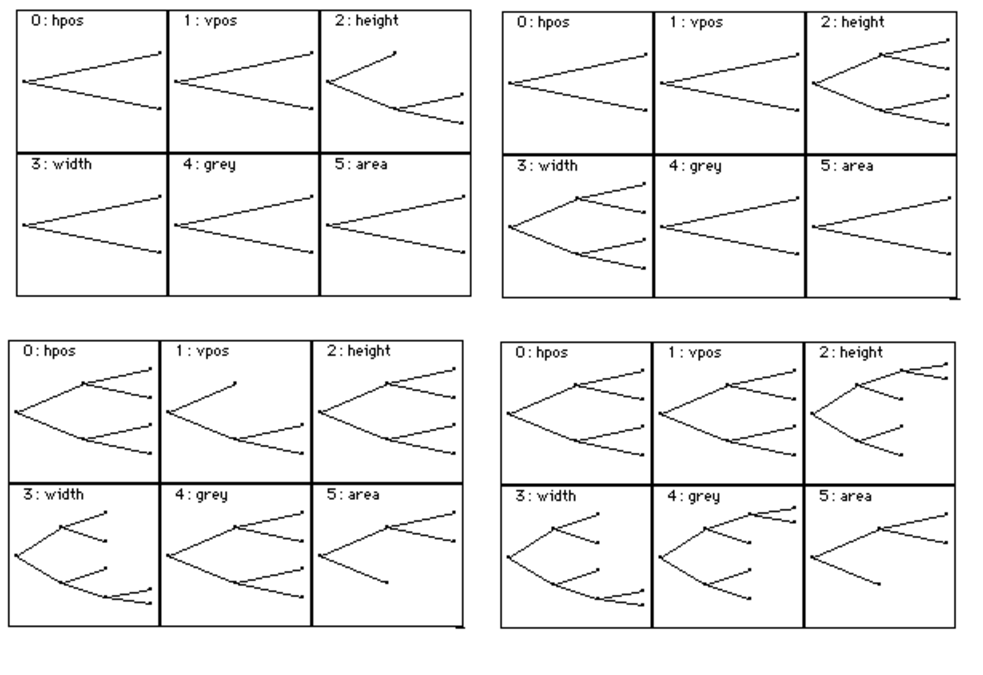
\includegraphics[width=\textwidth]{chap6/figs/gdis.pdf}}
\caption{\label{gdis1}Evolution of the discrimination
trees of {\bfshape  a1} (left) and {\bfshape  a2} (right).
Snapshots have been taken after 100 games (top) and 500 
games (bottom).} 
\end{figure}

Note that this simulation is very different from the 
ones shown in the previous chapter. The agents now get 
only feedback through overt selection of the referent. 
The hearer points to the identified referent and the speaker 
decides on the outcome of the game based on this 
non-verbal information, but speaker and hearer do not 
know whether they have used the same meaning or not. 
Very often there are alternative ways
to conceptualise reality, so even if agents would have
completely shared ontologies, there is still the possibility 
of guessing the wrong meaning. I have called this
the gavagai-problem, inspired by the philosopher
Quine, who tells the story of the anthropologist 
puzzled by the word `gavagai' uttered by a native 
in an undecoded language. Does `gavagai' mean rabit, animal 
scurrying by, the direction in which I will go 
now, or white furry object? 
The child who is acquiring a lexicon has
exactly the same problem. It explains why 
overextensions or underextensions
are seen in a child's first words. For example, 
the word for orange is applied to any small circular round 
object, including a ball, or a doorknob.

\subsection{Input-output coupling}

Obviously the first thing I had to do to get 
these results, is make the inputs of one layer the
outputs of the other (\figref{sieve2a}). When the 
speaker has conceptualised the scene, the possible
solutions enter the lexical layer for lexicon lookup. 
The resulting words get into a competition and the 
one with the highest score wins. In a more complete
system with a syntactic layer, different lexicalisations
would be considered by the syntactic layer to find 
the one that fits with the rest of the grammatical 
structure. 


\begin{figure}[htbp]
  \centerline{\includegraphics[width=.65\textwidth]{chap6/figs/sieve2a.pdf}}
\caption{\label{sieve2a}Flow of solutions through 
coupled layers from perception to conceptualisation and lexicalisation with re-entry links between them.} 
\end{figure}

The importance of having re-entry links now becomes\is{re-entrance}
clear. The choice which conceptualisation is finally chosen 
as the best one will depend on the lexical layer because 
the speaker should prefer those categories whose 
lexicalisation is best established, if he wants to 
maximise success in the game. Due to the constant evolution
of the lexicon and the presence of synonyms, the conceptual
layer cannot know once and for all what the most
appropriate conceptualisation from the viewpoint of 
language will be. And it needs to know the outcome of the
lexical layer to later update the scores of participating
categorisers. 

The hearer uses the same layers but now with solutions
flowing in the other direction. He gets a set of words
which generate possible conceptualisations through 
lexicon lookup and these then are applied to the 
scene to find the referent (\figref{sieve2b}). Because 
layers have this dual mode of operations, it is perfectly 
possible that the hearer has already guessed words and 
thus strong expectations based on the scene and his 
own conceptualisation of it, although this has not been
implemented in the Talking Heads yet. 


\begin{figure}[htbp]
  \centerline{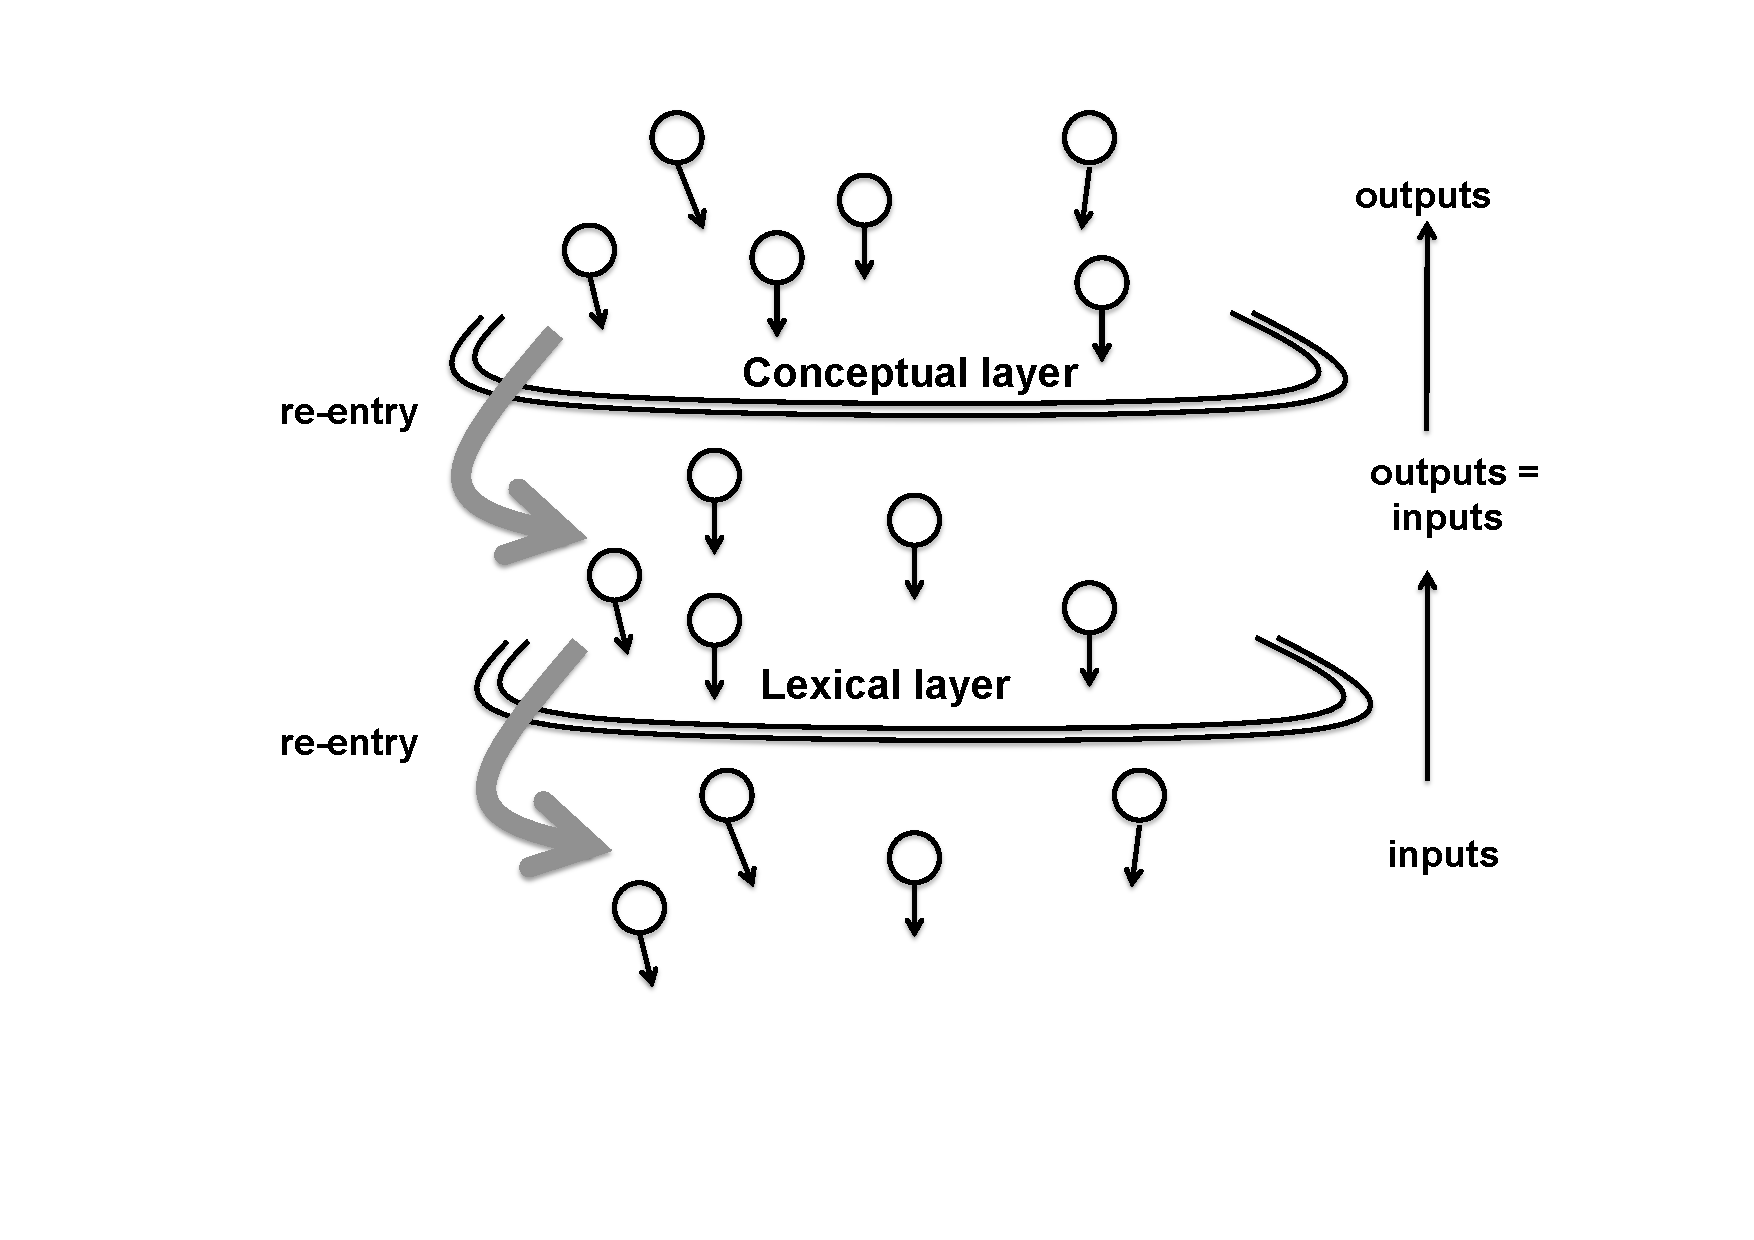
\includegraphics[width=.65\textwidth]{chap6/figs/sieve2b.pdf}}
\caption{\label{sieve2b}Layers operate in two 
directions. The flow of solutions in the hearer is shown from words to categories and perceptions
and in the other direction through re-entry.}
\end{figure}

Also for the hearer, the re-entrant flow is important. 
A hearer can only know which meaning was intended for a particular
word after trying out the meaning on the scene. He
therefore uses the context to determine the meaning of 
the utterance. For example, a particular word may mean both [LARGE]
and [DARK], particularly during the phase of 
early language acquisition. However if only one of these categories
picks out a single referent, it is chosen as 
the meaning, and the hearer will act upon this choice by 
pointing to the object it singles out from the scene. 

This architecture takes care of synonymy and ambiguity and
makes sure that the most plausible form/meaning/referent
chain stands out. A similar architecture may explain how
humans effortlessly pick out the appropriate meanings from 
the many possible meanings a word typically has and not even 
be aware of the alternatives. If our language sytems 
could not cope this way with ambiguity and ambiguity we 
would have had to use a lexicon where every word can 
have only a single meaning. Language has had to 
recruit whatever capacity was already available. 

\subsection{Updating the scores}

The next thing I had to do is reconsider the score
updating mechanisms, even though they are basically 
the same as used earlier (\figref{incr-decr2}). 
For a given referent, there are multiple meanings possible
(in case more than one channel is considered to 
be sufficiently salient), and
for each meaning there are multiple words. The best 
one of this whole lot is chosen by the speaker and used
for the utterance transmitted to the hearer. We have 
seen that it is important for the hearer to use lateral
inhibition based on the outcome of a game. But although 
the speaker is considering {\itshape all} the possible 
conceptualisations, lateral
inhibition should only take place between the 
lexicalisations of the meaning that was finally chosen. 
So when the game was successful, 
the speaker increases the association that was used with $\delta$
and decreases all the other associations
{\itshape with the same meaning}. $delta$ is still set to a reasonable
low value, namely $delta = 0.1$. 
The hearer does the same as explained earlier in 
the Naming Game. The score of all
the alternative meanings for the word (or words) 
that are used by the speaker are decreased. 
When the game fails, both the speaker and the hearer 
decrease the association that they used with $\delta$. No
change takes place to the scores of any of the 
other associations. 


\begin{figure}[htbp]
  \centerline{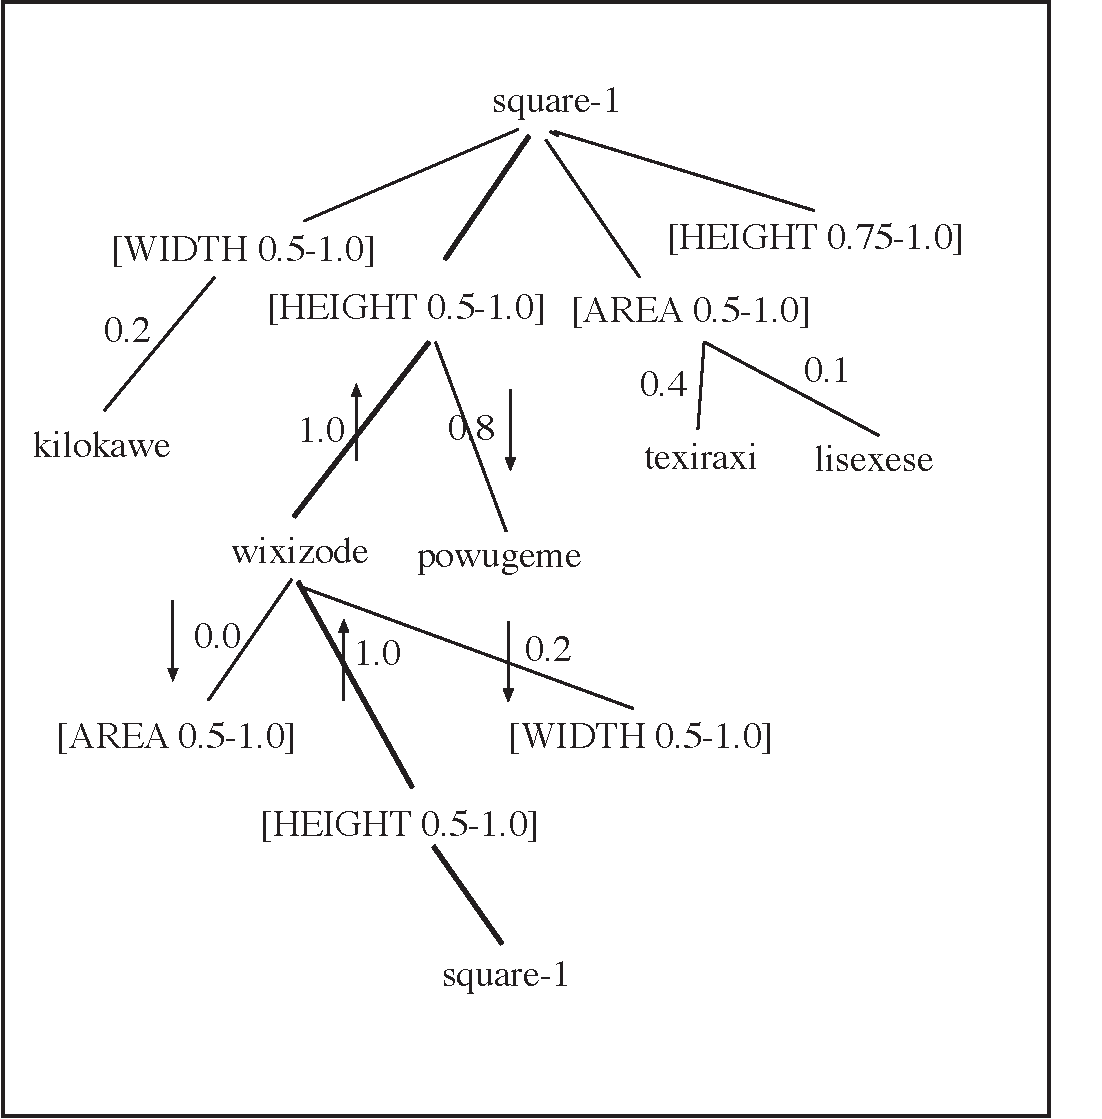
\includegraphics[width=.50\textwidth]{chap6/figs/incr-decr2.pdf}}
\caption{\label{incr-decr2}Score adjustments after a successful game. Used 
associations go up and competing associations go down.
The game producing these relationships is discussed
later as game 10008.}
\end{figure}

The scores of the categories and category
combinations in the discrimination trees should also 
be updated. When a category or category combination
is used as part of the communication 
in the game (as meaning for the speaker or
the hearer), its use counter goes up. When 
the game is successful, its success counter 
goes up. To know the score of a particular 
category or category-set, the agent simply 
divides success by use. Because the score of the categories 
thus depends on their success in the 
language game, a strong coordination gradually 
arises between conceptualisation and 
lexicalisations. After a while, categorisations
will be preferred that are amenable to yield
successful language games and of course the 
language only lexicalises categories that are 
nodes in discrimination trees. 
We thus get a progressive coordination of 
both the repertoire of categories and the 
lexicon, as I will discuss in more detail later. 

The other criteria discussed earlier (simplicity of 
the categories and level of depth in the tree) are 
still used for ranking the possible conceptualisations
coming out of the lexicon, particularly when none
of the meanings has been lexicalised yet or whether
there are multiple possibilities. The human brain 
is clearly capable to integrate many more criteria
in lexical choice. For example, when talking to a 
child we might use more common words than we would use 
when talking to another adult. 

\subsection{Repair processes}

Of course the other repair processes discussed earlier 
are still going on as well. Agents expand their 
discrimination trees when they fail to categorise and 
they invent new words or adopt words from the 
other if necessary. The task is more complicated compared
to the simple Naming Game because the hearer now gets
no direct feedback of the meaning only of the referent. 
In case of failure, the hearer must try to find himself a distinctive
category or category set discriminating the 
referent from the other objects in the context.

Here is an example game illustrating this
type of repair process. 
The data for game 77 (after sensor-scaling)
is shown in \tabref{tab:game77}. 


\begin{table}
\begin{center}
\begin{tabular}{ l  l  l  l  l  l  l }
\lsptoprule
{\itshape Obj} & Hpos & Vpos & Height & Width & Gray & Area \\ \midrule
0 & 0.51 & 0.98 & 0.90 & 0.47 & 0.79 & 0.60\\ 
1 & 0.75 & 0.68 & 0.26 & 0.09 & 0.14 & 0.20\\ 
2 & 0.76 & 0.54 & 0.56 & 0.26 & 0.94 & 0.36\\ 
\lspbottomrule
\end{tabular}
\caption{\label{tab:game77}Sensory data for game 77 after sensor-scaling.}
\end{center}
\end{table}
The speaker is again {\bfshape  a2}. HEIGHT is the most salient channel. 
{\bfshape  a2} has a word for [HEIGHT 0.75–1.0] (very tall), namely
`bowaluro', and uses it. The hearer {\bfshape  a1} 
does not know the 
word, conceptualises the scene, and arrives at the 
same category, so the hearer stores the new word
with the same meaning as the speaker. 
\begin{verbatim}
Game 77
  a2 is the speaker. a1 is the hearer. 
  a2 segments the context into 3 objects: 
       rectangle-0 rectangle-1 rectangle-2
  a2 chooses rectangle-1 as the topic 
  a2 categorises the topic as [HEIGHT 0.75–1.0]
  a2 says: `bowaluro'
  a1 does not know `bowaluro'
  a1 says: `bowaluro?'
  a2 points to rectangle-1
  a1 categorises the topic as [HEIGHT 0.75–1.0]
  a1 stores `bowaluro' as [HEIGHT 0.75–1.0]
\end{verbatim}
The reason why {\bfshape  a1} has guessed the right 
meaning of `bowaluro' is because both agents use
only the most salient channel and they both share
the same perception of reality. We will soon see 
that if these constraints are not valid, agents 
are not always so lucky and hence multiple meanings
start to circulate for the same word. 

A similar repair action takes place when the hearer
cannot guess a unique referent, as illustrated in
game 96 drawn from the same simulation series. 
The scene contains three rectangles and the 
topic is the most narrow rectangle. The segments in the scene of game 279
have the characteristics (after sensor-scaling) shown in \tabref{tab:279}. 


\begin{table}
\begin{center}
\begin{tabular}{ l  l  l  l  l  l  l }
\lsptoprule
{\itshape Obj}&Hpos&Vpos&Height&Width&Gray&Area \\ \midrule
0 &0.51 & 0.71 & 0.64 & 0.61 & 0.80 & 0.56\\ 
1 & 0.51 & 0.91 & 0.53 & 0.41 & 0.42 & 0.41 \\ 
\lspbottomrule
\end{tabular}
\caption{\label{tab:279}Sensory data for game 279.}
\end{center}
\end{table}
The hearer guessed the meaning used
by the speaker right away, because both 
share the same perception and both use the most 
salient channel as basis for categorisation. 
\begin{verbatim}
Game 96
  a1 is the speaker. a2 is the hearer. 
  a1 segments the context into 3 objects: 
       rectangle-0 rectangle-1 rectangle-2
  a1 chooses rectangle-1 as the topic 
  a1 categorises the topic as [WIDTH 0.0–0.25]
  a1 creates a new word: `kutaki'
  a1 says: `kutaki'
  a2 does not find a unique referent
  a2 says: `kutaki?'
  a1 points to rectangle-1
  a2 categorises the topic as [WIDTH 0.0–0.25]
  a2 stores `kutaki' as  [WIDTH 0.0–0.25]
\end{verbatim}

\section{Synonymy}

When we scale up the population, synonyms (several words\is{synonymy}
for the same meaning) will start to appear. Indeed,
when there are only two agents, the hearer picks 
up a word as soon as the speaker has created it. With a larger
group, it is much more likely that agents create words
not knowing that words already exist in the population, and 
it takes time for a new word to propagate. 

Synonyms are not a positive feature of a language. They make 
it less efficient for the speaker to find the most 
appropriate word to express a meaning, they require more
memory to store the lexicon, and confuse a new virgin 
agent coming into the group. In natural languages, synonyms get
damped and we have seen in the previous chapter
that the positive feedback loop between 
use and success (implemented by lateral inhibition
in the agent's score updating process) has the same
effect. Let us now see whether this is still the 
case if the hearer does not get any feedback about the
meaning used. 

The following simulation uses a group of ten agents. 
Each agent still only uses the most salient channel so that 
the agents can guess the meaning easily in case a word is not known. 
The evolution of communicative success for a series of 
4000 games, which means about 800 games per agent, 
is shown in \figref{gsucc2}. 
An effective lexicon and ontology is 
emerging because we see communicative success rise. 


\begin{figure}[htbp]
  \centerline{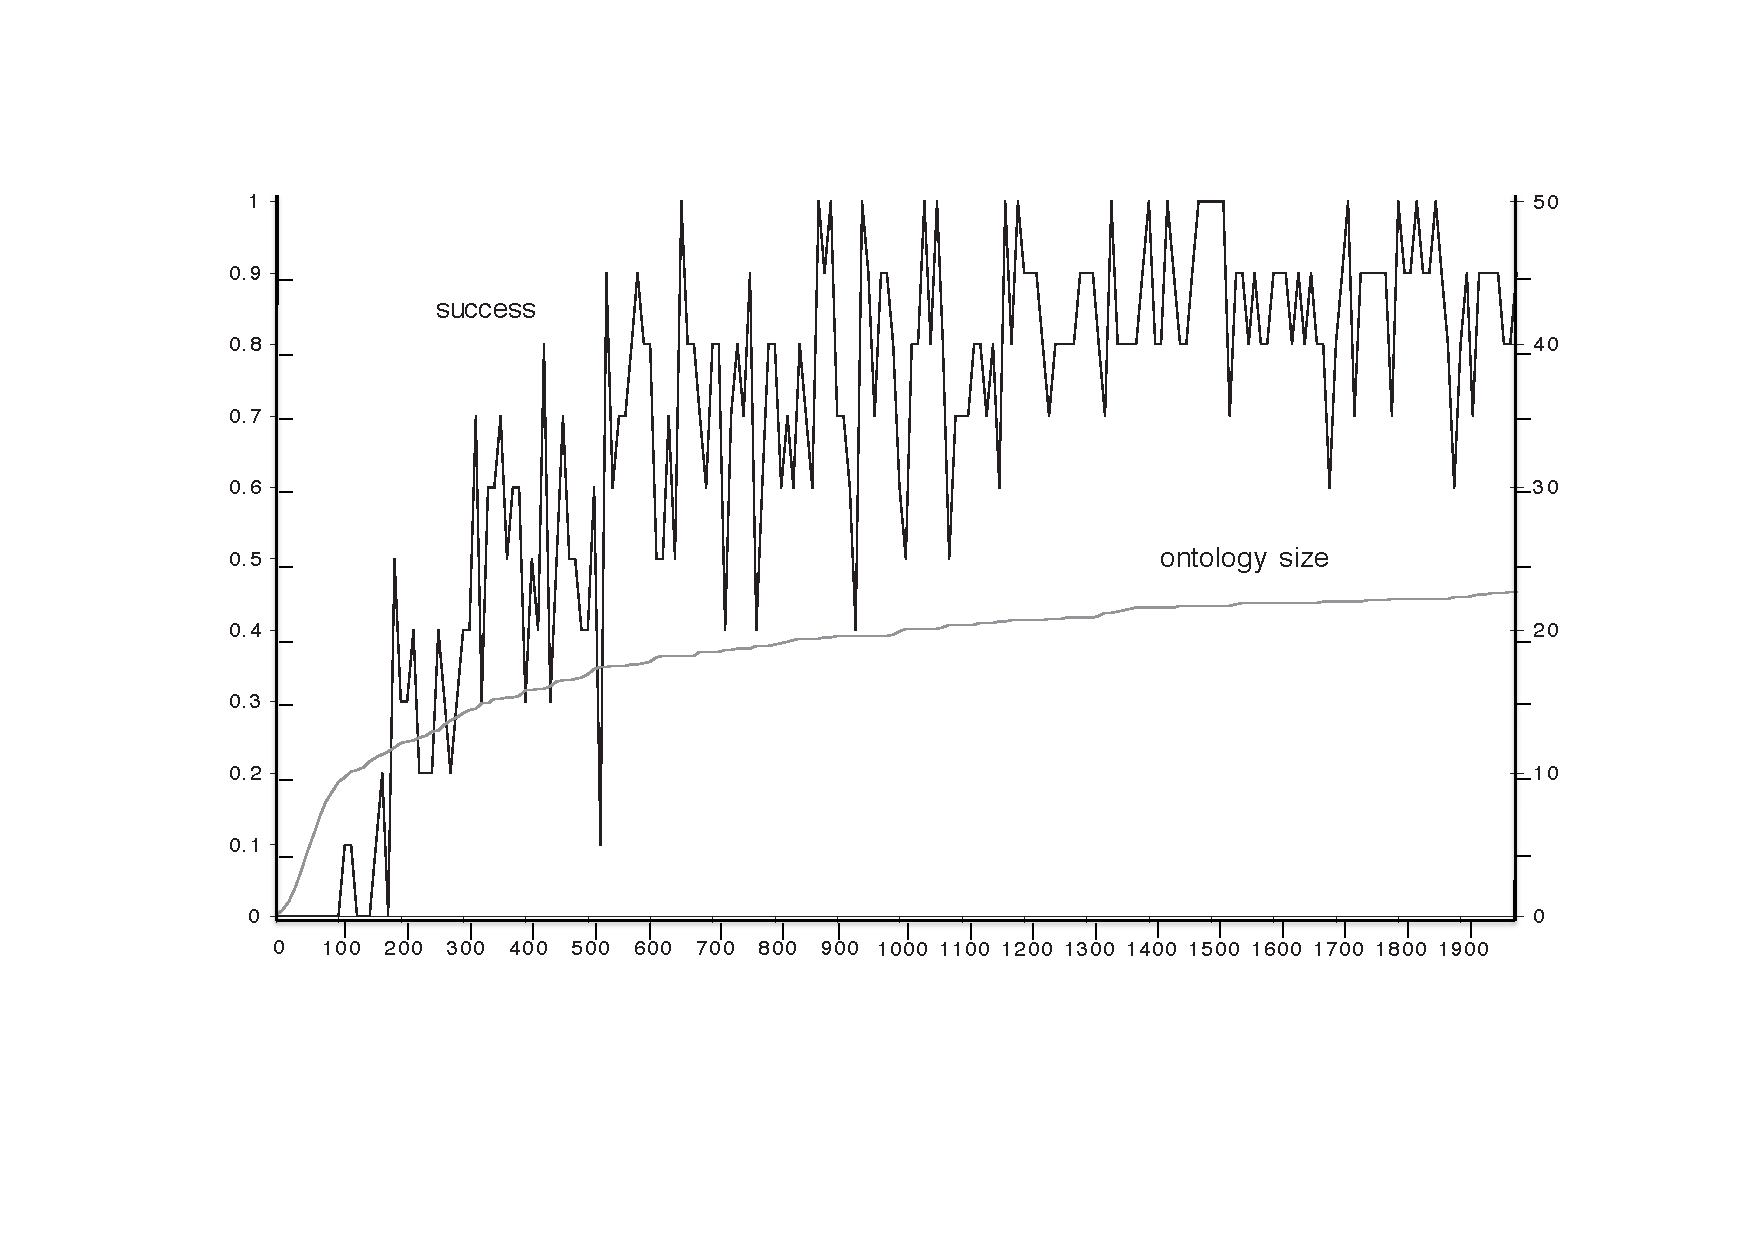
\includegraphics[width=\textwidth]{chap6/figs/gsucc2.pdf}}
\caption{\label{gsucc2}Communicative 
success (left y-axis) and average ontology size 
(right y-axis) is shown for a series of 4000
language games played by 10 agents.} 
\end{figure}

Part of the lexicons of five of the ten agents after 2000 games 
(only those words which have positive scores) are shown in the 
\tabref{tab:lex2000}. We see that synonymy does indeed occur. For
example, two words are in the 
running for [HPOS 0.5–1.0]: `rutaxese' and `xomupovi', and 
three for [VPOS 0.5–1.0]: `wavone', `zaxawe', and 
`dazofo'. Some words are already well established, for
example `numefuli' for [GRAY 0.5–1.0] (dark). 


\begin{table}
\begin{center}
\begin{tabular}{ l  l  l  l  l  l  l  }
\lsptoprule
{\itshape Meaning}&{\itshape Word}&{\bfshape  a1}&{\bfshape  a2}&{\bfshape  a3}&{\bfshape  a4}&{\bfshape  a5} \\ \midrule
{}[HPOS 0.5–1.0]&rutaxese& &0.1& & &\\ 
 & xomupovi&0.1& &0.2& &0.1\\ 
{}[VPOS 0.5–1.0]&wavone& & &0.3& &\\ 
 & zaxawe& & & &0.1& \\ 
 & dazofo&0.1& & &0.2&\\ 
{}[WIDTH 0.0–0.5]&buxevo& & & & & \\ 
 & vubupo&1.0&0.6&1.0&0.1&1.0\\ 
{}[WIDTH 0.5–1.0]&pawixona& & &0.1& & \\ 
 & rikepule&1.0&0.8&1.0&1.0&1.0\\ 
{}[WIDTH 0.5–0.75]&gowinoge& & &0.1& &  \\ 
 & wesurodi& & & &0.2&\\ 
{}[WIDTH 0.75–1.0]&besabi& & &0.2& & \\ 
 & lituvi&0.1& & & & \\ 
{}[GRAY 0.5–0.75]&goxomixe& &0.1& & & \\ 
 & korufo& & & &0.2&\\ 
{}[GRAY 0.0–0.5]&numefuli&1.0&0.7&1.0&1.0&1.0\\ 
{}[GRAY 0.0–0.25]&rekemaxi&0.2& & & & \\ 
{}[GRAY 0.5–1.0]&faluleru&0.6&0.6&1.0&1.0&1.0\\ 
 & nupanu& & & & &0.2 \\ 
\lspbottomrule
\end{tabular}
\caption{\label{tab:lex2000}Lexicon of five agents after 2000 games.}
\end{center}
\end{table}

The positive feedback loop between use and success
has already dampened some synonyms. For some cases, like [GRAY 0.5–1.0] the competition has died out 
with one word `faluleru' being the winner. 
For others, like [HPOS 0.5–1.0], the competition 
is still going on, although we can guess
that `xomupovi' is probably going to be the winner. 

It is instructive to follow the history of the words 
in use for a particular meaning. For 
example, let us look at the words for [GRAY 0.5–1.0] 
(dark) in the very early phases of lexicon development.
Three different words are quickly created, and 
`faluleru' is the first one that has some success. 
\begin{verbatim}
Game 76
 Speaker a4 creates `notabefe' for [GRAY 0.5–1.0]
 Hearer a5 adopts `notabefe' for [GRAY 0.5–1.0]
Game 79 
 Speaker a2 creates `vivevobo' for [GRAY 0.5–1.0]
 Hearer a7 does not adopt `vivebo' 
     (failed to discriminate)
Game 88 
 Speaker a7 creates `faluleru' for [GRAY 0.5–1.0]
 Hearer a4 adopts `faluleru' for [GRAY 0.5–1.0]
Game 100 
 Speaker a7 uses `faluleru' for [GRAY 0.5–1.0]
 Hearer a4 correctly interprets `faluleru'
\end{verbatim}
The semiotic triangles existing at this point in the population are 
summarised in \figref{triangle6}. 
Agent {\bfshape  a4} is now already in a dilemma because he has created
`notabefe' and picked up `faluleru' from {\bfshape  a7}. 


\begin{figure}[htbp]
  \centerline{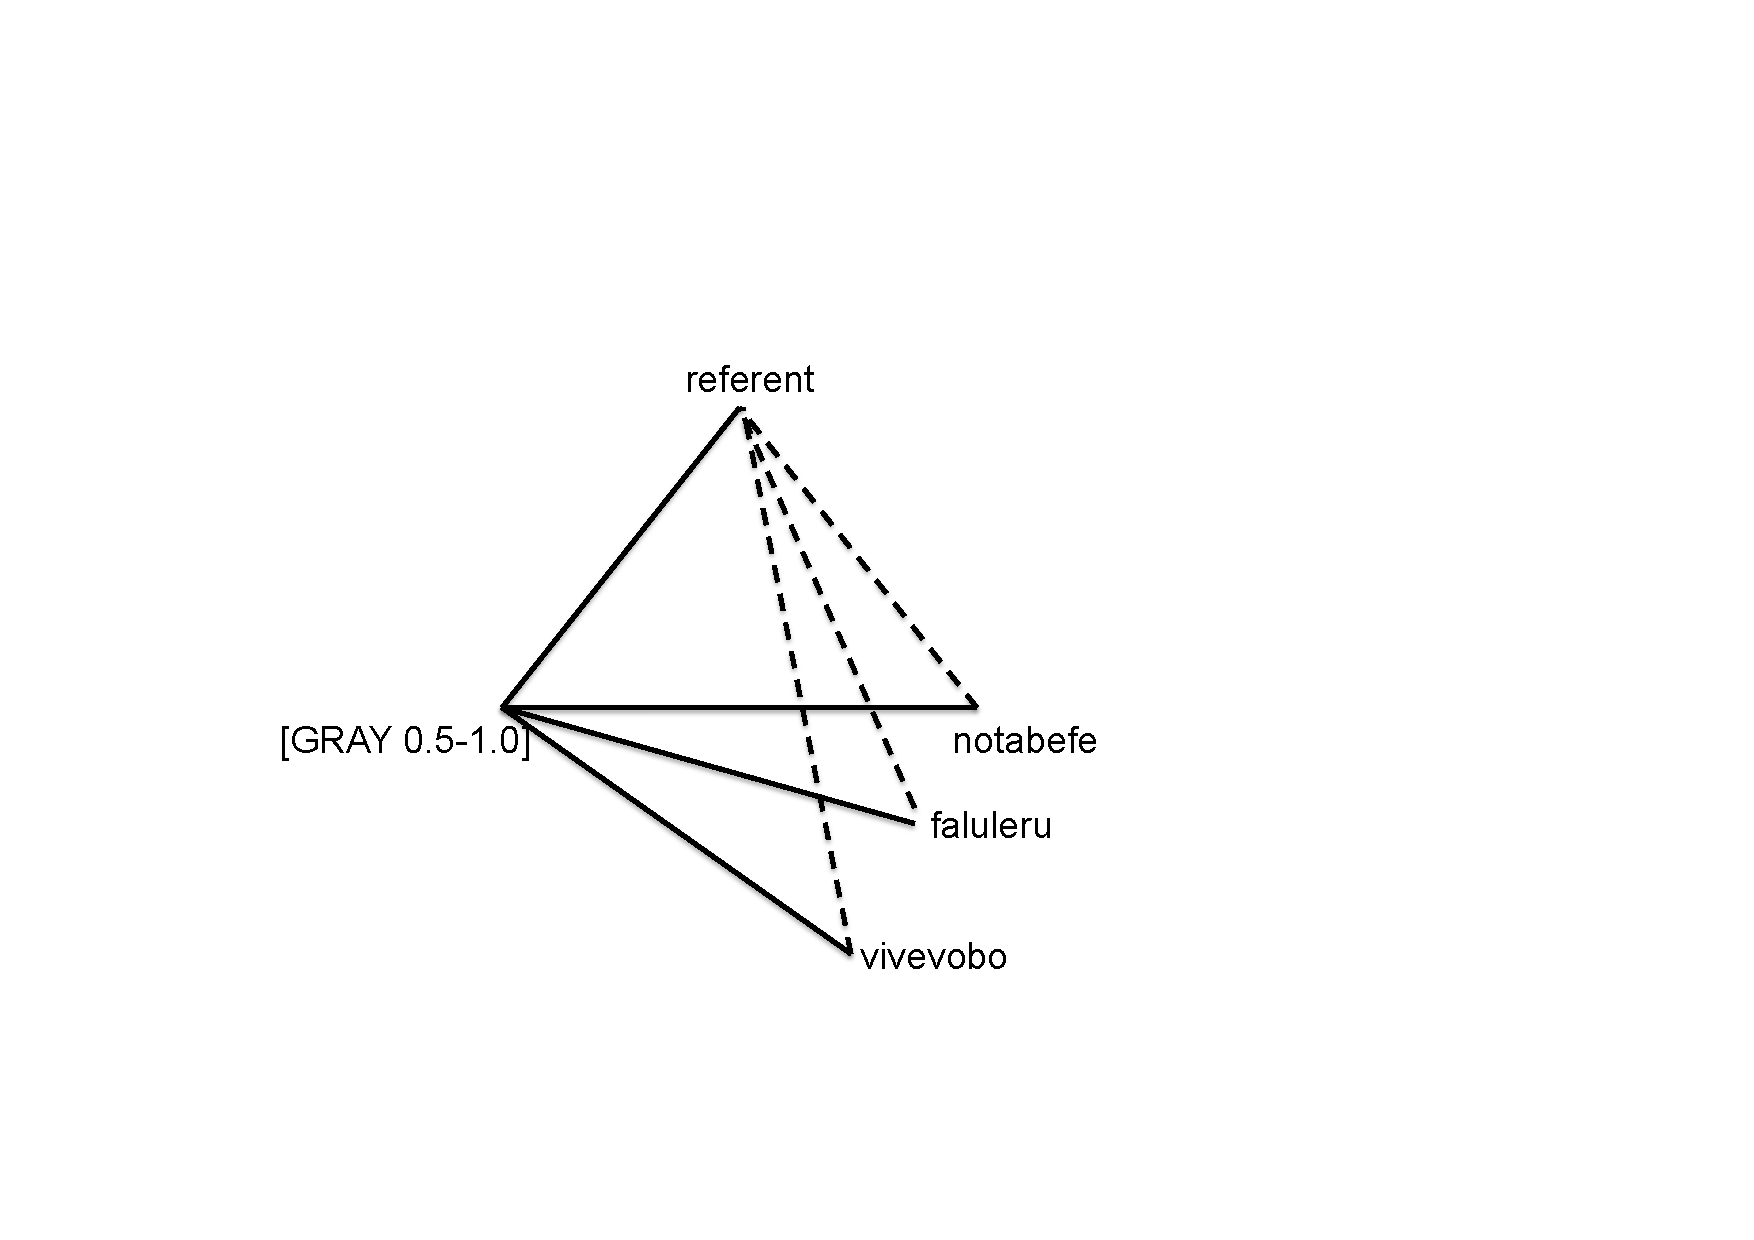
\includegraphics[width=.50\textwidth]{chap6/figs/triangle6.pdf}}
\caption{\label{triangle6}In the case of synonymy, 
there are multiple words for the same meaning and hence the 
same referent.}
\end{figure}

With a lower word creation rate ($w_{c}$), 
fewer new words would be created. The initial bootstrapping
of the lexicon would then take a bit longer but the 
process of weeding out synonymy would be shorter. 
With a lower word adoption rate ($w_{a}$), agents are
less inclined to adopt a word and that again diminishes
the chance that new words spread, if words already 
exist for the same meaning. But even with high word creation
and word adoption rates, the whole system stabilises automatically. 
The stronger a lexicon is already in place, the fewer
new synonyms arise because new words
created by virgin agents entering the population have hardly 
any chance to propagate. 

Note that the word creation 
rate can never be completely zero because then the agents
would no longer be able to handle new meanings. The word 
adoption rate can never be equal to zero either because then 
new words cannot spread in the population and there
would be a high chance that the lexicon does not become coherent
with subgroups getting stuck with different
words for the same meaning. 

Because there are synonyms, agents must now choose
which word to use. The one with the highest
score should clearly be preferred because based on the
evidence the agent has gathered so far, this
gives the highest chance of success in the game. {\bfshape  a4}
is faced with this kind of choice in 
the next game in the series involving the meaning
{}[GRAY 0.5–1.0]. {\bfshape  a4} chooses `faluleru' because this 
word has the highest score. It is immediately picked up by 
{\bfshape  a1}: 
\begin{verbatim}
Game 101
  a4 is the speaker. a1 is the hearer. 
  a4 segments the context into 2 objects: 
       rectangle-0 rectangle-1
  a4 chooses rectangle-1 as the topic 
  a4 categorises the topic as [GRAY 0.5–1.0]
  a4 has two words for [GRAY 0.5–1.0]:
       `faluleru' (0.20)
       `notabefe' (0.00)
  a4 says: `faluleru'
  a1 does not know `faluleru'
  a1 says: `faluleru?'
  a4 points to rectangle-1
  a1 categorises the topic as [GRAY 0.5–1.0]
  a1 stores `faluleru' as [GRAY 0.5–1.0]
\end{verbatim}
After this game, three agents `know' the word 
`faluleru' for [GRAY 0.5–1.0]: {\bfshape  a4}, {\bfshape  a1}, 
and {\bfshape  a7}. When we continue to inspect the
simulation we see that `notabefe' takes a bit of 
a revenge. The next games with the 
meaning [GRAY 0.5–1.0] all involve the word `notabefe': 
\begin{verbatim}
Game 111
 Speaker a5 uses `notabefe' for [GRAY 0.5–1.0]
 Hearer a4 correctly interprets `notabefe'
Game 113
 Speaker a4 uses `notabefe' for [GRAY 0.5–1.0]
 Hearer a9 adopts `notabefe' for [GRAY 0.5–1.0]
Game 127
 Speaker a9 uses `notabefe' for [GRAY 0.5–1.0]
 Hearer a6 adopts `notabefe' for [GRAY 0.5–1.0]
\end{verbatim}
But then there is another occurrence of `faluleru': 
\begin{verbatim}
Game 135 
 Speaker a1 uses `faluleru' for [GRAY 0.5–1.0]
 Hearer a2 adopts `faluleru' for [GRAY 0.5–1.0]
\end{verbatim}
And now {\bfshape  a6}, which has not been involved 
yet in any interaction concerning the 
meaning [GRAY 0.5–1.0], further confuses the situation by 
creating a new word, `sopine', which {\bfshape  a5}, playing
the role of hearer, adopts. 
\begin{verbatim}
Game 140
 Speaker a6 creates `sopine' for [GRAY 0.5–1.0]
 Hearer a5 adopts `sopine' for [GRAY 0.5–1.0]
\end{verbatim}
This kind of evolution continues with a struggle between 
`notabefe' and `faluleru'. The agents know both 
words so the games do not fail. But `faluleru', 
just by chance, starts to occur a bit more often
which causes its score to go up a bit more. 
This results in `faluleru' being used even more, 
and, due to lateral inhibition, `notabefe' used 
less. Gradually `faluleru' dominates for 
the whole population. 
After 2000 games, the competitors to `faluleru' have 
all disappeared from the group lexicon. 

\section{Ambiguity} 

We now continue in small steps to scale up the\is{ambiguity}
challenge to the agents by progressively 
adding more realism to the simulation. So far I 
assumed that agents use only 
the most salient channel for categorising the topic
and that their perception of the world is identical.
Consequently a hearer can guess with 100 \% success the
meaning of an unknown word and 
it is therefore no wonder that the agents arrive at a 
shared communication system, 
even though neither the lexicon nor the repertoire
of categories has been supplied in advance by a 
designer nor their development centrally
coordinated. The main problem for them so far is 
the rise of synonyms which need to be damped to 
increase the probability of successful and 
efficient communication. 

I now relax the saliency assumption. When 
there is a lower saliency threshold, more than one
sensory channel is considered by the conceptual 
layer, possibly leading to several alternative
conceptualisations of the scene. The question is 
then whether the agents are still able to reach 
a shared communication system despite the unavoidable
word ambiguities that this generates. 

We begin again by looking at simulations
with two agents so that we 
can clearly see the impact of multiple conceptualisations. 
The architecture of the agents has not changed, I only 
lowered the saliency treshold. 
The scenes have become a bit more complex as well. They 
now not only contain rectangles but also squares, circles, 
and triangles. This has a limited impact because the 
same sensory channels are used as before and none of them 
is really sensitive to shape properties. 


\begin{figure}[htbp]
  \centerline{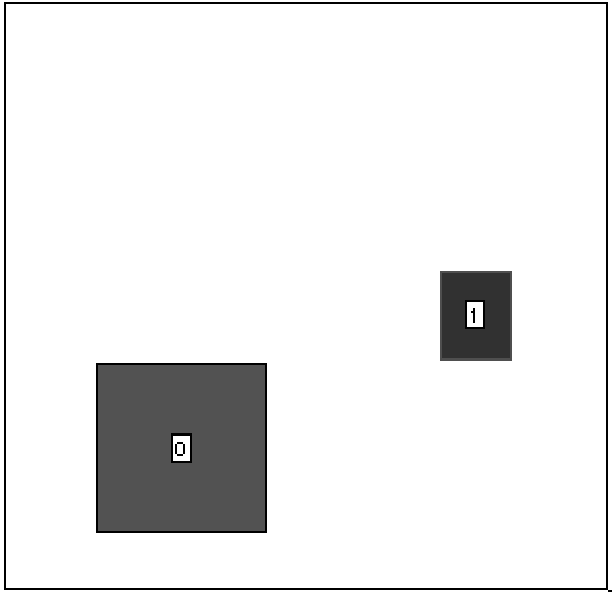
\includegraphics[width=.40\textwidth]{chap6/figs/scene-game3.pdf}}
\caption{\label{scene-game3}Scene used
in game 3.}
\end{figure}

\subsection{How words may still get the same meaning}

When inspecting the simulation results, we see                          
first of all that 
we may still accidentally get the same situation
as before, i.e. one where the hearer selects 
the same channel as the speaker for conceptualising 
the scene, even though several channels 
are salient. This happens in the
following game which involves a scene with a rectangle
and a square (\figref{scene-game3}). 

The data for game 3, after sensor-scaling,
are shown in \tabref{tab:game3}. 


\begin{table}
\begin{center}
\begin{tabular}{ l  l  l  l  l  l  l }
\lsptoprule
{\itshape Obj} & Hpos & Vpos & Height & Width & Gray & Area \\ \midrule
0 & 0.37 & 0.44 & 0.92 & 0.92 & 0.69 & 0.10\\ 
1 & 0.98 & 0.55 & 0.25 & 0.11 & 0.78 & 0.88\\ 
\lspbottomrule
\end{tabular}
\caption{\label{tab:game3}Sensory data for game 3 after scaling.}
\end{center}
\end{table}
Values for VPOS and GRAY are very close so they are not 
considered as sufficiently salient.
\begin{verbatim}
Game 3
  a1 is the speaker. a2 is the hearer. 
  a1 segments the context into 2 objects: 
       square-0 rectangle-1 
  a1 chooses rectangle-1 as the topic 
  a1 considers as salient AREA WIDTH HEIGHT HPOS 
  a1 categorises the topic as [HEIGHT 0.0–0.5]
  a2 creates a new word: `mibati'
  a1 says: `mibati'
  a2 does not know `mibati'
  a2 says: `mibati?'
  a1 points to rectangle-1
  a1 considers as salient AREA WIDTH HEIGHT HPOS 
  a1 categorises the topic as [HEIGHT 0.0–0.5]
  a1 stores `mibati' as [HEIGHT 0.0–0.5]
\end{verbatim}
{}[HEIGHT 0.0–0.5] has been chosen by the speaker
because HEIGHT was one of the salient channels (even 
though clearly not the only salient one) and 
because a successful distinction already existed in 
the ontology. The same 
distinction was chosen by chance by the hearer, but he 
could just as well have chosen a distinction based on 
the AREA, WIDTH or HPOS. 

In the next game of the simulation series, `mibati'
is used again, now by {\bfshape  a2} as speaker. It is 
based on a scene with a triangle and a rectangle.
The data for game 4 are shown in \tabref{tab:mibati} (after scaling).  


\begin{table}
\begin{center}
\begin{tabular}{ l  l  l  l  l  l  l }
\lsptoprule
{\itshape obj} & HPOS & VPOS & HEIGHT & WIDTH & GRAY & AREA \\ \midrule
0 & 0.47 & 0.23 & 0.90 & 0.83 & 0.49 & 0.34\\ 
1 & 0.21 & 0.22 & 0.67 & 0.79 & 0.86 & 0.63\\ 
\lspbottomrule
\end{tabular}
\caption{\label{tab:mibati}Lexicon of a1 and a2 after 500 games.}
\end{center}
\end{table}
The rectangle is chosen as topic. Two alternative
categories can be used by {\bfshape  a2} (and are listed
by the commentator) but the one preferred
is the one with the strongest lexicalisation, which is 
`mibati'.
\begin{verbatim}
Game 4
  a2 is the speaker. a1 is the hearer. 
  a2 segments the context into 2 objects: 
       triangle-0 rectangle-1
  a2 chooses rectangle-1 as the topic 
  a2 considers as salient AREA GRAY HEIGHT HPOS 
  a2 categorises the topic as [HEIGHT 0.0–0.5] 
{}[GRAY 0.5–1.0]
  a2 has the word
       mibati for [HEIGHT 0.0–0.5] (1.0)
  a2 says: `mibati'
  a1 interprets `mibati' as [HEIGHT 0.0–0.5]
  a1 points to rectangle-1
  a2 signals OK 
\end{verbatim}

This example illustrates two points. First of all the 
language interpretation process influences 
which conceptualisation of the scene is preferred. For 
the speaker, both [HEIGHT 0.0–0.5] (short) and [GRAY 0.5–1.0]
(dark) are possible ways to distinguish the topic from the 
other objects in the context. But [HEIGHT 0.0–0.5] is 
chosen because its lexicalisation has a higher score. 
Second, we begin to see why agents will manage to 
coordinate their ontologies, even though they do not 
have any direct feedback about each other's internal 
structures. The score of [HEIGHT 0.0–0.5] goes up after
this game and if the 
agent has to choose a category later purely based on 
the score of the categories themselves, [HEIGHT 0.0–0.5] will 
be the one being preferred. Unless [GRAY 0.5–1.0] manages
to become successfully lexicalised itself, it even risks to 
get pruned away. 


\begin{figure}[htbp]
  \centerline{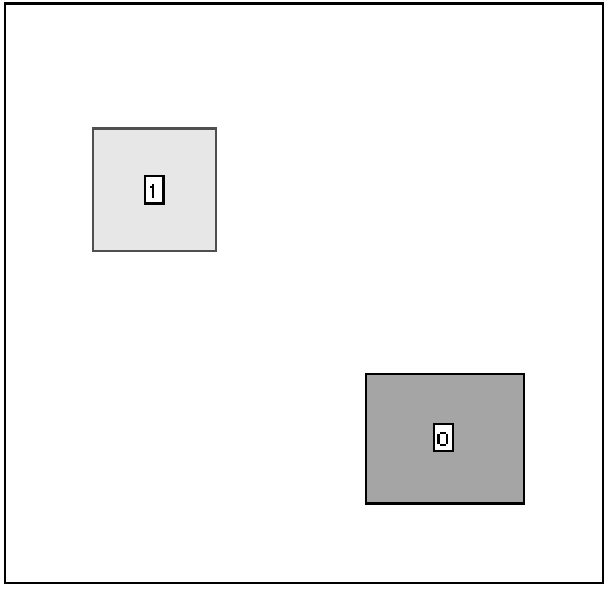
\includegraphics[width=.40\textwidth]{chap6/figs/scene-game9.pdf}}
\caption{\label{game9}Scene used
in game 9. Square-1 is the topic. Several conceptualisations are 
possible so the agents get divergent meanings.}
\end{figure}


\begin{figure}[htbp]
  \centerline{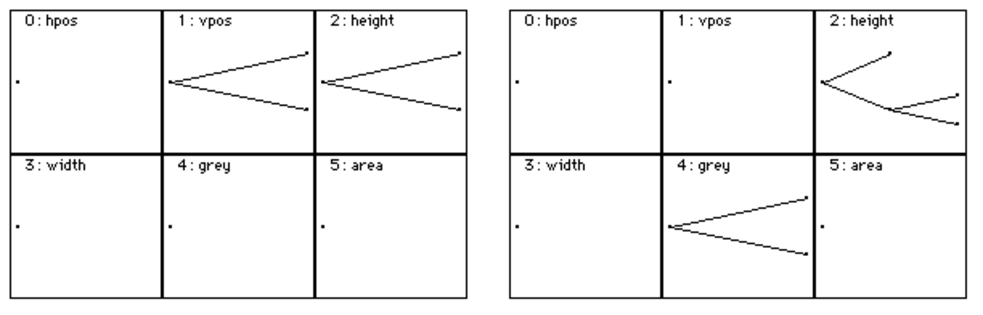
\includegraphics[width=\textwidth]{chap6/figs/discri-game9.pdf}}
\caption{\label{discri-game9}Discrimination trees
of speaker a1 (left) and hearer a2 (right) available 
in game 9}
\end{figure}

\subsection{How words get different meanings}

Here is an example where ambiguity slips in 
the lexicon. The game involves two 
objects: a rectangle and a square (\figref{game9}). 
The data for game 9, after sensor-scaling, are
shown in \tabref{tab:different}.  


\begin{table}
\begin{center}
\begin{tabular}{ l  l  l  l  l  l  l }
\lsptoprule
{\itshape obj} & HPOS & VPOS & HEIGHT & WIDTH & GRAY & AREA \\ \midrule
0 & 0.92 & 0.38 & 0.59 & 0.83 & 0.36 & 0.61\\ 
1 & 0.32 & 0.88 & 0.54 & 0.54 & 0.12 & 0.42\\ 
\lspbottomrule
\end{tabular}
\caption{\label{tab:different}Data for game 9 after sensor-scaling.}
\end{center}
\end{table}
The discrimination trees of the two agents at this point
are shown in \figref{discri-game9}. 
The speaker uses a distinction based on the 
VPOS channel namely [VPOS 0.5–1.0] (top), creates
a word for it `puxazi', and transmits this to the hearer. 
The hearer does not know the word,
conceptualises the scene based on this non-verbal
hint from the speaker, and identifies the category
{}[GRAY 0.0–0.5] (light) as distinctive. So this 
meaning is stored and it is different from the one used by 
speaker. The current constellation of meanings
is summarised in \figref{triangle4}. 
\begin{verbatim}
Game 9
  a1 is the speaker. a2 is the hearer. 
  a1 segments the context into 2 objects: 
       rectangle-0 square-1 
  a1 chooses square-1 as the topic 
  a1 considers as salient GRAY WIDTH VPOS HPOS 
  a1 categorises the topic as [VPOS 0.5–1.0]
  a2 creates a new word: `puxazi'
  a1 says: `puxazi'
  a2 does not know `puxazi'
  a2 says: `puxazi?'
  a1 points to square-1
  a2 considers as salient GRAY WIDTH VPOS HPOS 
  a2 categorises the topic as [GRAY 0.0–0.5]
  a2 stores `puxazi' as [GRAY 0.0–0.5]
\end{verbatim}


\begin{figure}[htbp]
  \centerline{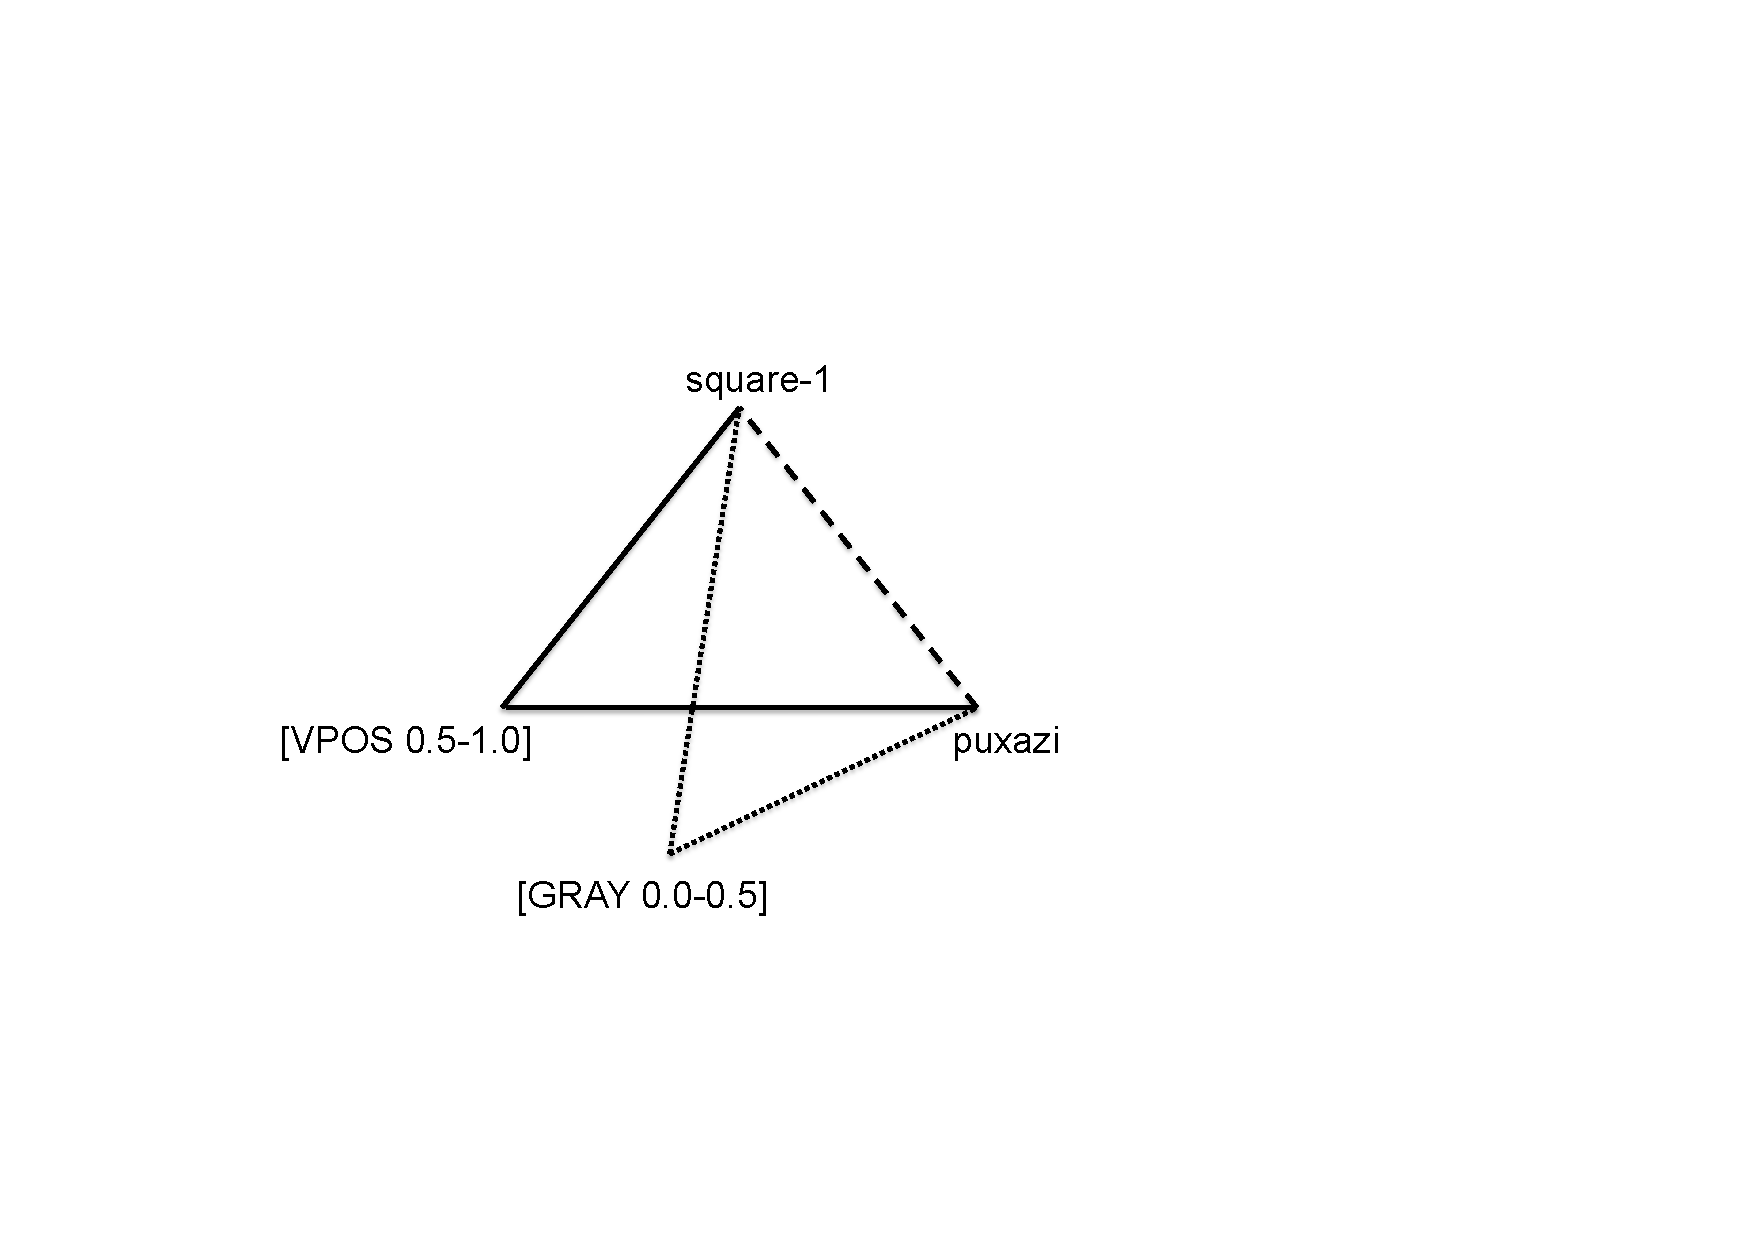
\includegraphics[width=.45\textwidth]{chap6/figs/triangle4.pdf}}
\caption{\label{triangle4}Semiotic triangles
underlying game 9. For the same referent and the same word, 
there are two different meanings. Dashed lines indicate
the relations used by the speaker {\bfshape  a2}. Straight lines
indicate those used by the hearer {\bfshape  a1}.}
\end{figure}

A subsequent game (game 11) illustrates that despite 
semantic incoherence, a game can still succeed. The agents 
do not know that each of them means something else by 
`puxazi' and if the meanings are compatible, they 
have no reason to change their internal lexicon:
\begin{verbatim}
Game 11
  a2 is the speaker. a1 is the hearer. 
  a2 segments the context into 3 objects: 
       circle-0 rectangle-1
  a2 chooses rectangle-1 as the topic 
  a2 considers as salient AREA GRAY WIDTH HPOS 
  a2 categorises the topic as [GRAY 0.0–0.5]
  a2 says: `puxazi'
  a1 interprets `puxazi' as [VPOS 0.5–1.0]
  a1 points to rectangle-1
  a2 signals OK 
\end{verbatim}



\begin{figure}[htbp]
  \centerline{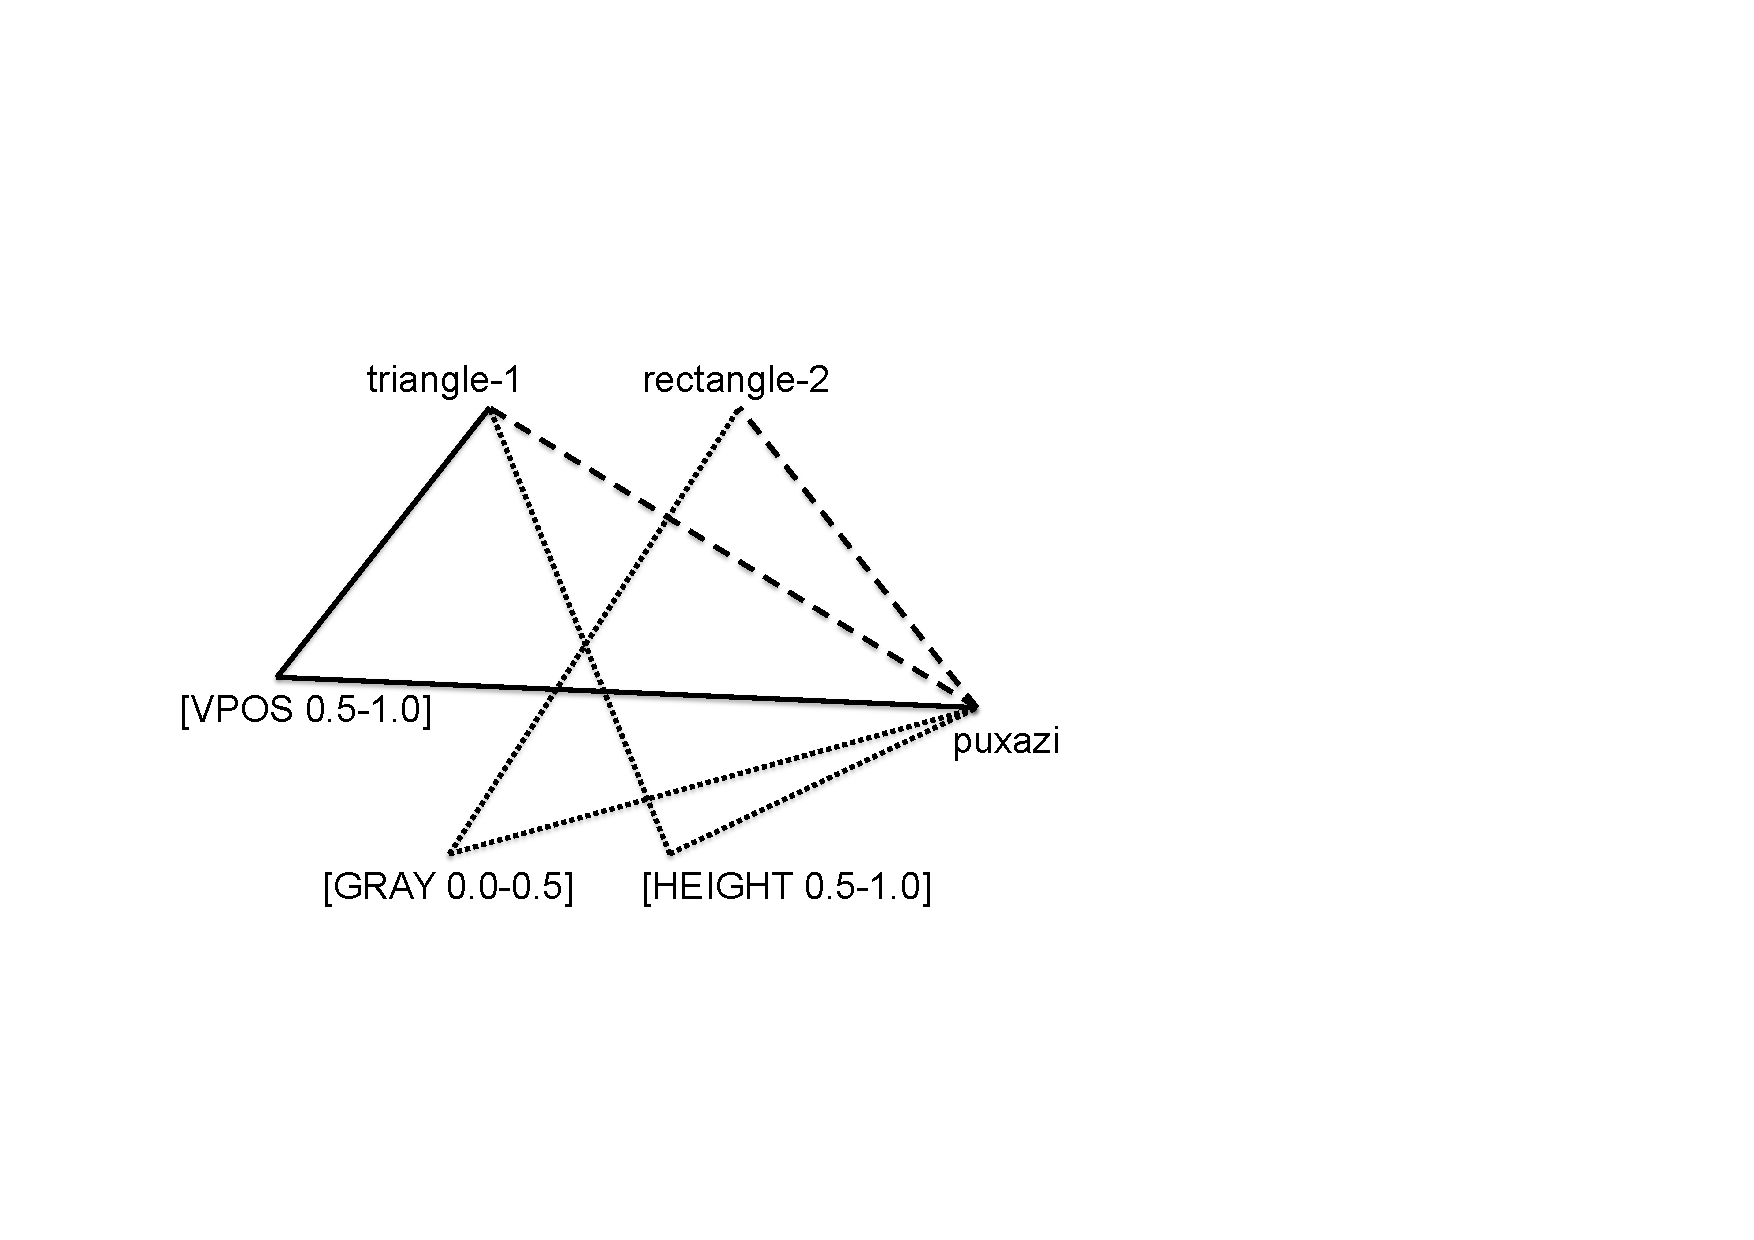
\includegraphics[width=.60\textwidth]{chap6/figs/triangle3.pdf}}
\caption{\label{triangle3}Semiotic triangles used in
game 14. Dashed lines are the relations used by 
the hearer {\bfshape  a2}. Straight lines those of the 
speaker {\bfshape  a1}. After this game, {\bfshape  a1}
adopts yet another meaning for `puxazi', namely 
{}[HEIGHT 0.5–1.0].}
\end{figure}
Here is next a game (game 14) where {\bfshape  a2} comes to adopt 
the other meaning of `puxazi', because the first
meaning does not work in the present context. 
The game involves three objects: two rectangles and a 
triangle (\figref{scene-game14}).
The data for game 14, before context scaling, are
shown in \tabref{tab:game14}. 


\begin{table}
\begin{center}
\begin{tabular}{ l  l  l  l  l  l  l }
\lsptoprule
{\itshape obj} & HPOS & VPOS & HEIGHT & WIDTH & GRAY & AREA \\ \midrule
0 & 0.60 & 0.49 & 0.12 & 0.09 & 0.78 & 0.06\\ 
1 & 0.95 & 0.71 & 0.51 & 0.60 & 0.07 & 0.15\\ 
2 & 0.29 & 0.31 & 0.29 & 0.65 & 0.03 & 0.33\\ 
\lspbottomrule
\end{tabular}
\caption{\label{tab:game14}Sensory data for game 14 after scaling.}
\end{center}
\end{table}

{\bfshape  a1} conceptualises the scene using 
{}[VPOS 0.5–1.0], which he has lexicalised as `puxazi'. 
For {\bfshape  a2}, `puxazi' means [GRAY 0.0–0.5] (light), but this 
meaning identifies both rectangle-2 and
triangle-1 (\figref{triangle3}). The game therefore
fails and the speaker points to the topic. The hearer
conceptualises the scene based on this non-verbal
hint from the speaker using the HEIGHT dimension and adopts this as the second meaning 
of `puzaxi'. 
\begin{verbatim}
Game 14
  a1 is the speaker. a2 is the hearer. 
  a1 segments the context into 3 objects: 
       rectangle-0 triangle-1 rectangle-2
  a1 chooses triangle-1 as the topic 
  a1 considers as salient HEIGHT VPOS HPOS 
  a1 categorises the topic as 
{}[VPOS 0.5–1.0] [HEIGHT 0.5–1.0]
  a1 says: `puxazi'
  a2 interprets `puxazi' as [GRAY 0.0–0.5]
  a2 identifies rectangle-2 triangle-1
  a2 says: `puxazi?'
  a1 points to triangle-1
  a2 considers as salient HEIGHT VPOS HPOS 
  a2 categorises the topic as [HEIGHT 0.5–1.0]
  a2 stores `puxazi' as [HEIGHT 0.5–1.0]
\end{verbatim}
Note that the hearer could in principle 
also have categorised the
scene using VPOS and HPOS, because they are
equally salient. So there was absolutely no 
guarantee that `puxazi' would have been associated 
with [HEIGHT 0.5–1.0] by {\bfshape  a2}. Moreover {\bfshape  a2} stores
an association between `puxazi' and [HEIGHT 0.5–1.0], even though 
there is already another word for 
{}[HEIGHT 0.5–1.0] in his lexicon. The fact that 
several meanings are possible to distinguish the topic in a given 
context has not only the consequence that ambiguity
arises but also that synonyms may enter into the lexicon, 
even with only two agents!


\begin{figure}[htbp]
  \centerline{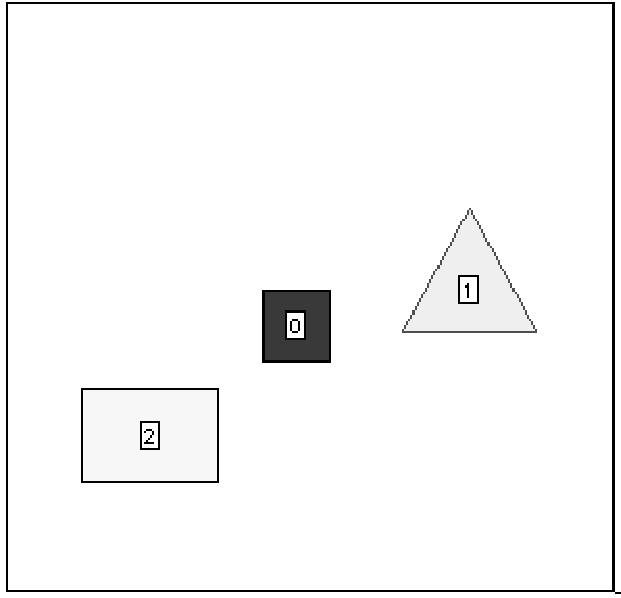
\includegraphics[width=.40\textwidth]{chap6/figs/scene-game14.pdf}}
\caption{\label{scene-game14}Scene used
in game 14. Synonymy arises because the hearer conceptualises
the scene differently from the speaker.}
\end{figure}

\subsection{Competition between word meanings }

Once a word has more than one meaning (ambiguity), 
and once several words exist for the same meaning 
(synonymy), a struggle between word-meaning
pairs sharing the same word or the 
same meaning develops. The lateral inhibition carried out by the 
speaker in case of a successful game pushes
down alternative lexicalisations for the same meaning, 
thus damping synonyms, and the lateral inhibition carried out 
by the hearer pushes down alternative meanings for the 
same word, thus damping ambiguity. 


\begin{figure}[htbp]
  \centerline{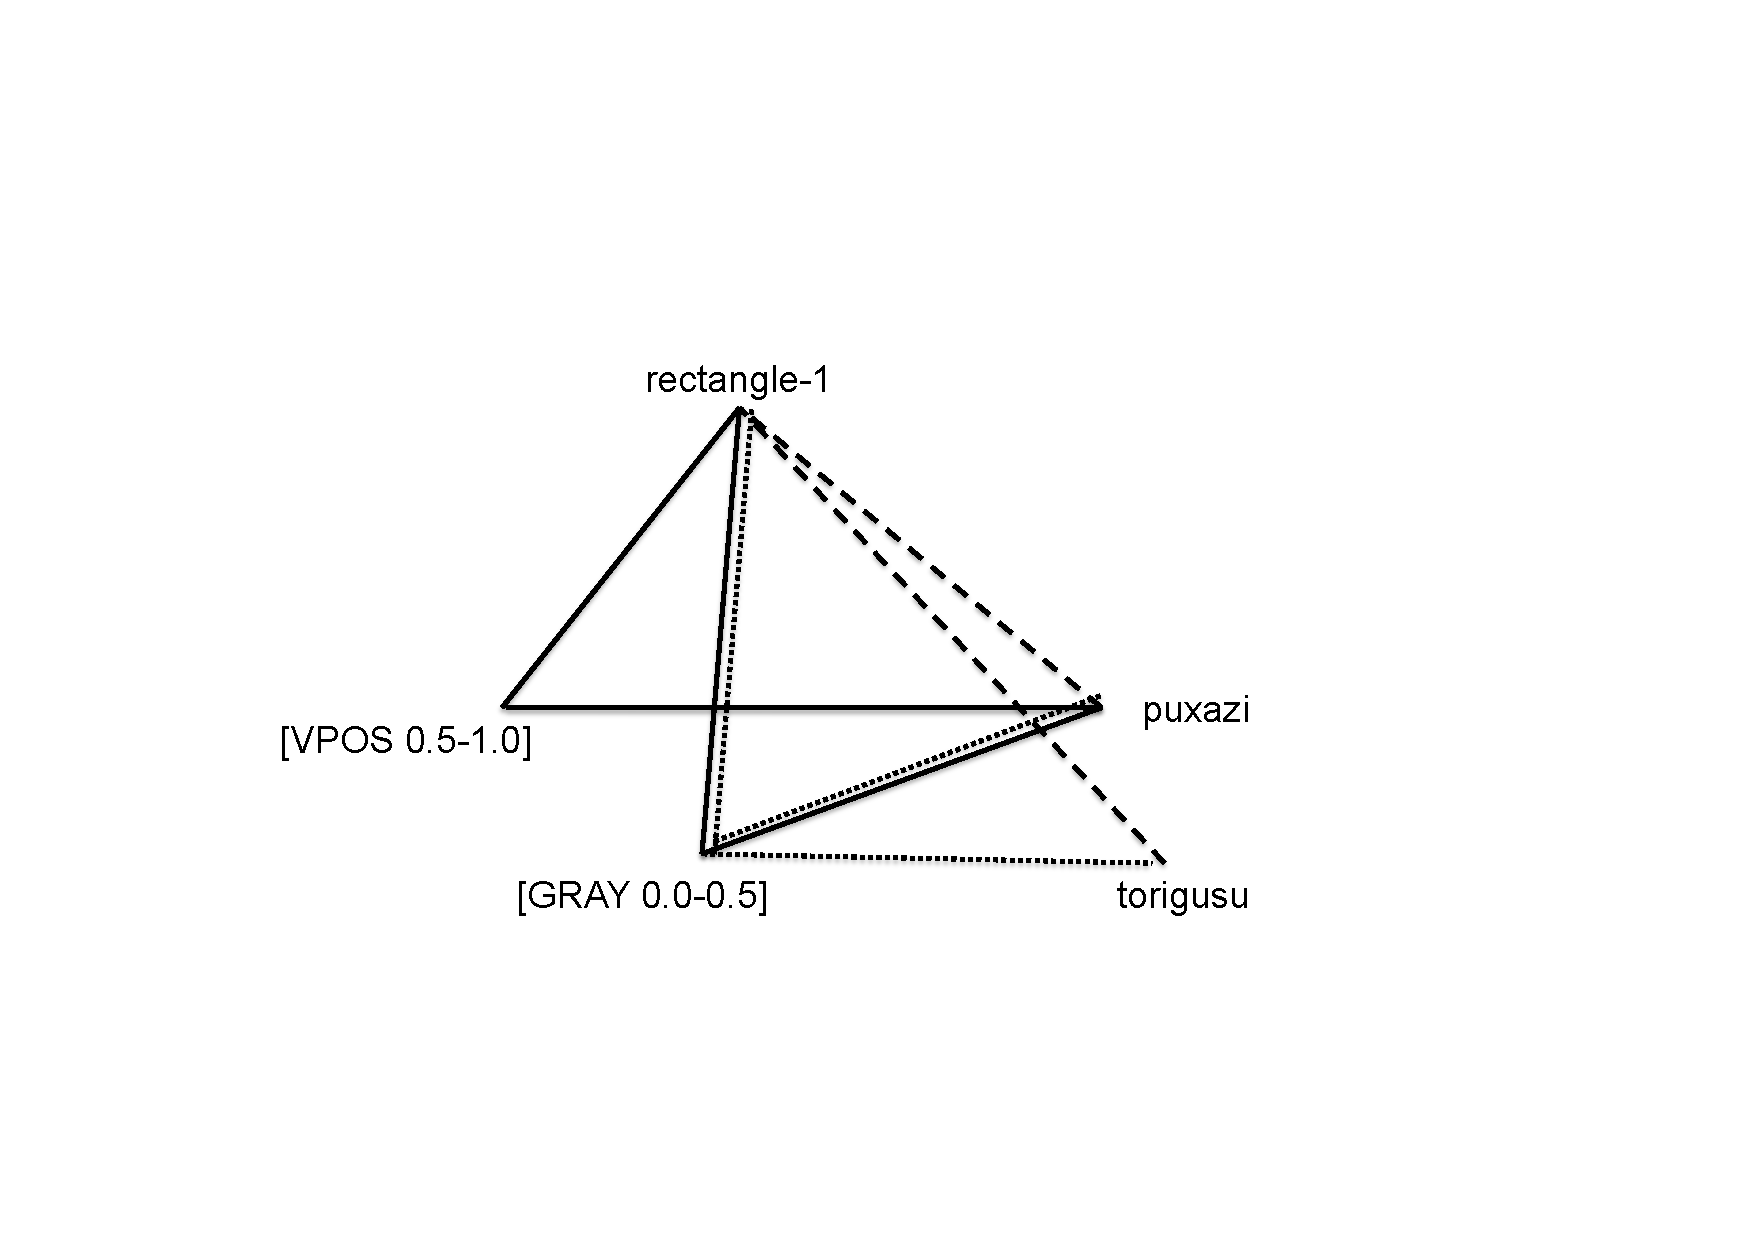
\includegraphics[width=.60\textwidth]{chap6/figs/triangle5.pdf}}
\caption{\label{triangle5}Semiotic triangles used 
in game 25. The score of the relation between [GRAY 0.0–0.5] and 
`puxazi' is increased in both agents. The relation between `puxazi' and 
{}[GRAY 0.0–0.5] gets damped.}
\end{figure}

Game 25 illustrates this effect of 
lateral inhibition. The situation before the game is 
as depicted in \figref{triangle5}. 
Two words (with different meanings) are competing in {\bfshape  a2} to 
identify the referent: `puxazi' (meaning 
{}[GRAY 0.0–0.5], i.e. light) and `torigusu'
(meaning [VPOS 0.0–0.5], i.e. lower).  `puxazi' has
a higher score and wins the competition. Because the game 
was successful, the score
of `puxazi' goes up. The score of `torigusu' 
does not change because it concerns another 
meaning. Two meanings for `puxazi'
are competing in {\bfshape  a1}: [GRAY 0.0–0.5] (light)
and [VPOS 0.0–0.5] (down). [VPOS 0.0–0.5] gets damped and 
the score of [GRAY 0.0–0.5] goes up, thus helping to 
further disambiguate `puxazi'. 
\begin{verbatim}
Game 25
  a2 is the speaker. a1 is the hearer. 
  a2 segments the context into 2 objects: 
       rectangle-0 rectangle-1 
  a2 chooses rectangle-1 as the topic 
  a2 considers as salient GRAY VPOS
  a2 categorises the topic as [VPOS 0.0–0.5] 
{}[GRAY 0.0–0.5] [GRAY 0.0–0.25]
  a2 has the words
       puxazi for [GRAY 0.0–0.5] (0.20)
       torigusu for [VPOS 0.0–0.5] (0.0)
  a2 says: `puxazi'
  a1 interprets `puxazi' as
{}[GRAY 0.0–0.5] (0.20)
{}[VPOS 0.0–0.5] (0.0)
  a1 points to rectangle-1
  a2 signals OK
\end{verbatim}
After this game, the assocation between [GRAY 0.0–0.5] 
and `puxazi' will have a score of 0.3 in both agents. 
The association between `puxazi' and [VPOS 0.0–0.5] 
in the hearer is decreased, but because it was already 
0.0, it cannot decrease further. 

Note that the speaker not only conceptualises the scene using 
the most generic distinctions ([GRAY 0.0–0.5], 
{}[VPOS 0.0–0.5]) but also
with more specific ones ([GRAY 0.0–0.25]). Indeed it 
may happen that there is no word for a more generic 
distinction, but there is one for a more specific 
one, in which case it should be used. 
So, all discriminative distinctions, 
whatever their level of detail, are
transmitted from the categorisation layer to the 
lexical layer and it is up to the lexical layer
to choose. Of course, everything else being equal, 
other criteria are still important. If there is a 
more abstract category (meaning one higher in the 
discrimination tree) it is preferred over a more 
specific one if they have equal lexical scores. 

\subsection{Lexical and ontological development} 

Despite the additional complication of mutually 
compatible meanings for unknown words, the two agents
nevertheless manage to 
build up a shared communication system, as can be seen 
from \figref{gsucc3}. Each time the ontology is 
extended, communicative success dips because a new 
word needs to be acquired, but the agents clearly 
manage to become successful in the guessing game. 



\begin{figure}[htbp]
  \centerline{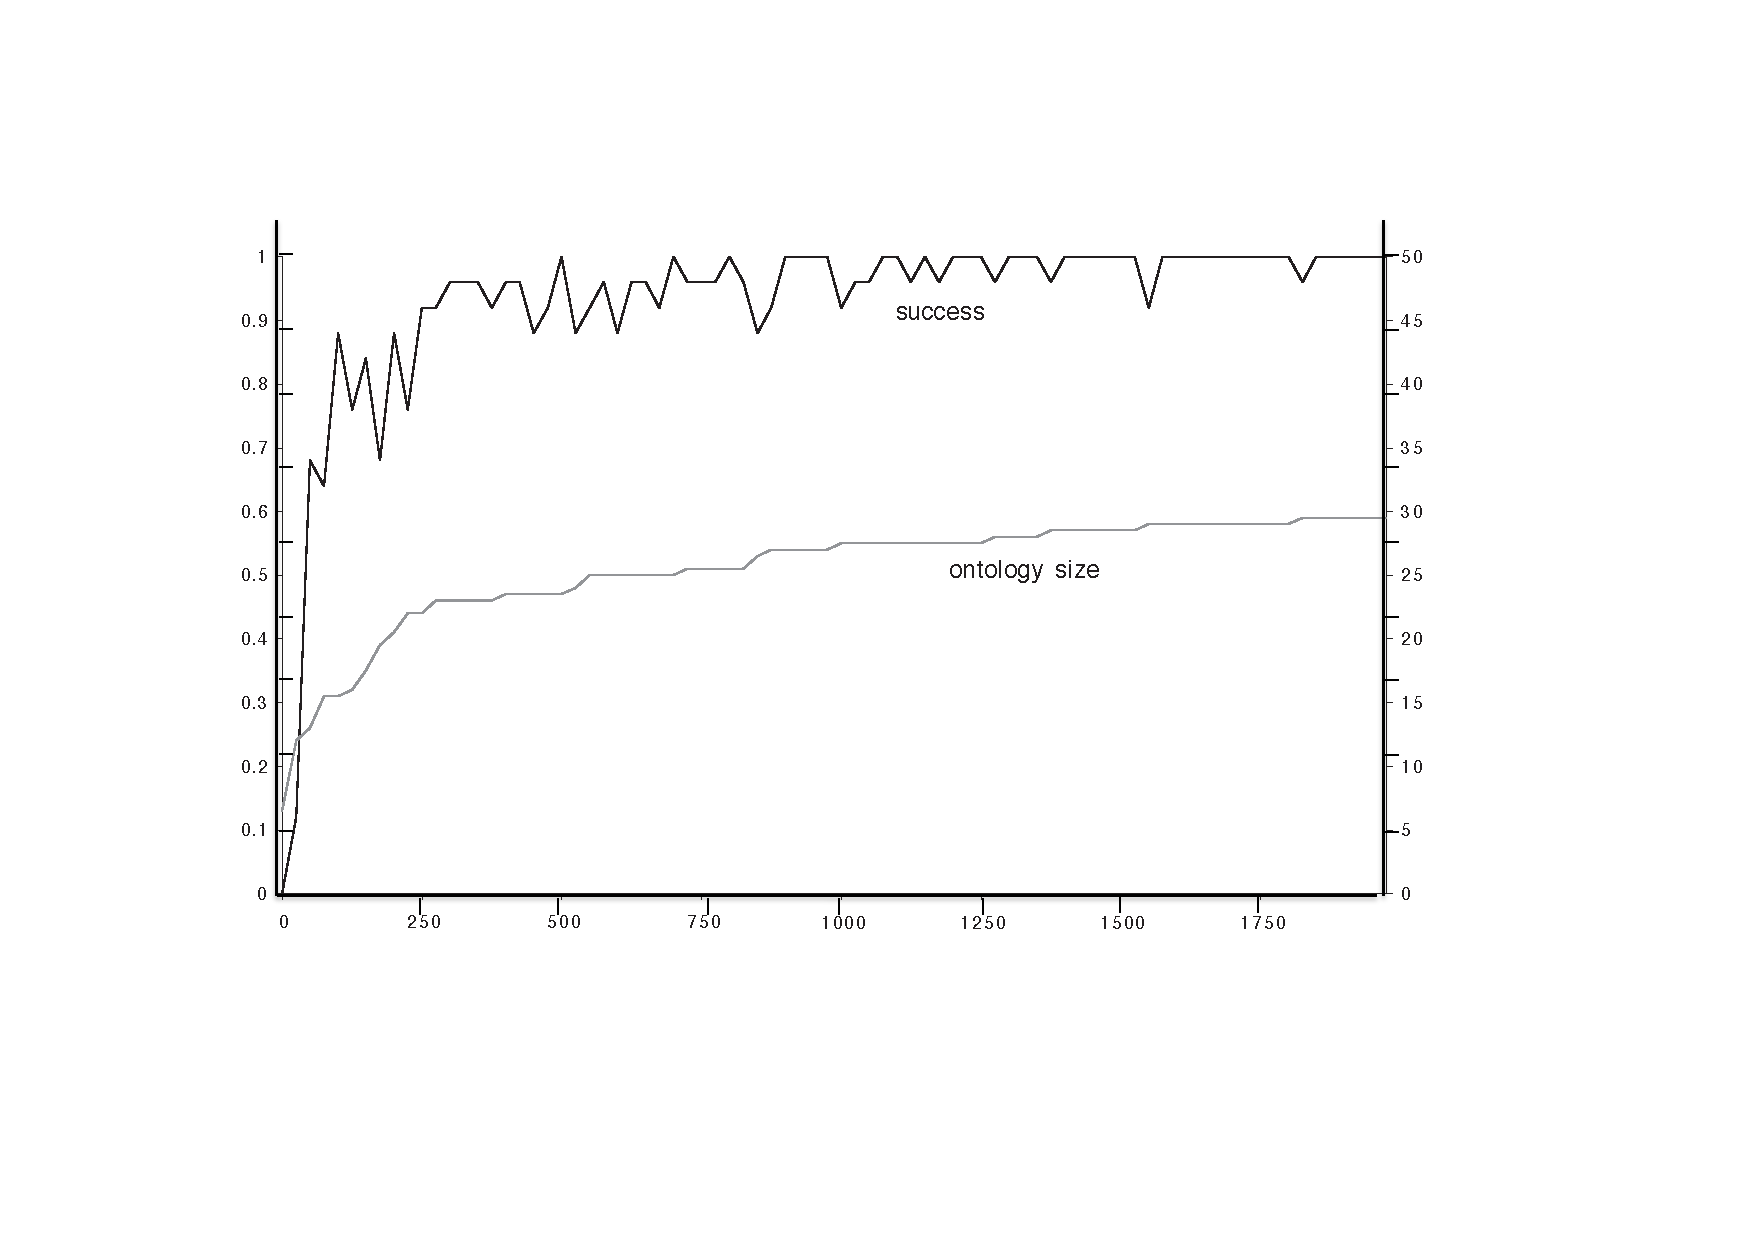
\includegraphics[width=\textwidth]{chap6/figs/gsucc3.pdf}}
\caption{\label{gsucc3}Communicative 
success (left y-axis) and average ontology size 
(right y-axis) for a series of 2000
language games played by two agents.} 
\end{figure}
Success does not mean that the lexicons are completely 
identical. As we have seen in game 11, it is possible
to have communicative success with different 
meanings for the same word as long as the different meanings
pick out the same referent. Of course in the domain of
the GEOM world, it is a pure coincidence that two categories
pick out the same referent and therefore alternative 
meanings for the same word will get damped. However, if there
are more regularities, ambiguity persists much longer. 
In fact, ambiguity may persist in natural languages if 
the different meanings of a word are so 
closely related that it is sufficiently often unclear
which meaning is intended. 

Here are some snapshots of the developing lexicon. 
After 30 games, the lexicon of the established
words (i.e. associations with a score greater 
than 0.0 for at least one agent) is as in \tabref{tab:after30}. 



\begin{table} 
\begin{center}
\begin{tabular}{ l  l  l  l  l }
\lsptoprule
{\itshape Meaning}&{\itshape Word}&{\itshape Translation} & {\bfshape  a1}&{\bfshape  a2} \\ \midrule
{}[VPOS 0.0–0.5] &torigusu&left&0.4&0.3\\ 
{}[HEIGHT 0.0–0.5]&mibati&short &0.6&0.6\\ 
{}[HEIGHT 0.5–1.0]&puxazi&tall &0.2&0.0\\ 
{}[GRAY 0.0–0.5]& puxazi&light &0.6&0.7\\ 
{}[GRAY 0.25–0.5]&turawa&medium light&0.1&0.0\\ 
{}[GRAY 0.5–1.0]& xubevilo&dark &0.0&0.1\\ 
\lspbottomrule
\end{tabular}
\caption{\label{tab:after30}Group lexicon after 30 games.}
\end{center}
\end{table}

Note that there are two meanings for `puxazi': 
{}[GRAY 0.0–0.5] (light) and [HEIGHT 0.5–1.0] (tall). 

The lexicon after 200 games is shown in \tabref{tab:after200}. 


\begin{table} 
\begin{center}
\begin{tabular}{ l  l  l  l  l }
\lsptoprule
{\itshape Meaning}&{\itshape Word}&{\itshape Translation} & {\bfshape  a1}&{\bfshape  a2} \\ \midrule
{}[HPOS 0.0–0.5] &lefividi&left&0.2&0.2\\ 
{}[HPOS 0.5–1.0] &vuvovo&right&0.2&0.4\\ 
{}[VPOS 0.0–0.5] &torigusu&left&0.8&0.2\\ 
{}[VPOS 0.5–1.0] &rugomoto&right&1.0&1.0\\ 
{}[HEIGHT 0.0–0.5]&mibati&short &1.0&0.9\\ 
{}[GRAY 0.0–0.5]& puxazi&light &0.3&0.6\\ 
{}[GRAY 0.25–0.5]&turawa&medium light&0.4&0.4\\ 
{}[GRAY 0.5–1.0]& xubevilo&dark &0.4&0.5\\ 
{}[GRAY 0.5–0.75]& visuxa&very dark &0.3&0.3\\ 
\lspbottomrule
\end{tabular}
\caption{\label{tab:after200}Group lexicon after 200 games.}
\end{center}
\end{table}

The second meaning of `puxazi' has now disappeared
from the lexicon. So we basically see the same situation 
as before when only one most salient channel was
considered by the agents. Words for more general distinctions
happen to be lexicalised first because they are more 
often useful in the game, but when needed words for more specific
meanings start to develop. 

\section{Scaling up}

Conforted by having reached a new plateau in 
the challenges confronting the agents, I now go 
one more step further. First we scale up the 
population to see whether despite the ambiguity
now persistently present, a larger group of 
agents still manages to develop a shared
communication system. 

\subsection{Increasing the population size}

We already know from the previous section that 
a larger population automatically increases
the risk for synonymy. \figref{agnt10} shows the 
evolution of communicative success and average
ontology size in a population
of ten agents. We see again a steady progression
towards an effective communication system. Recall that 
these games are played with randomly generated scenes
from the GEOM world. 


\begin{figure}[htbp]
  \centerline{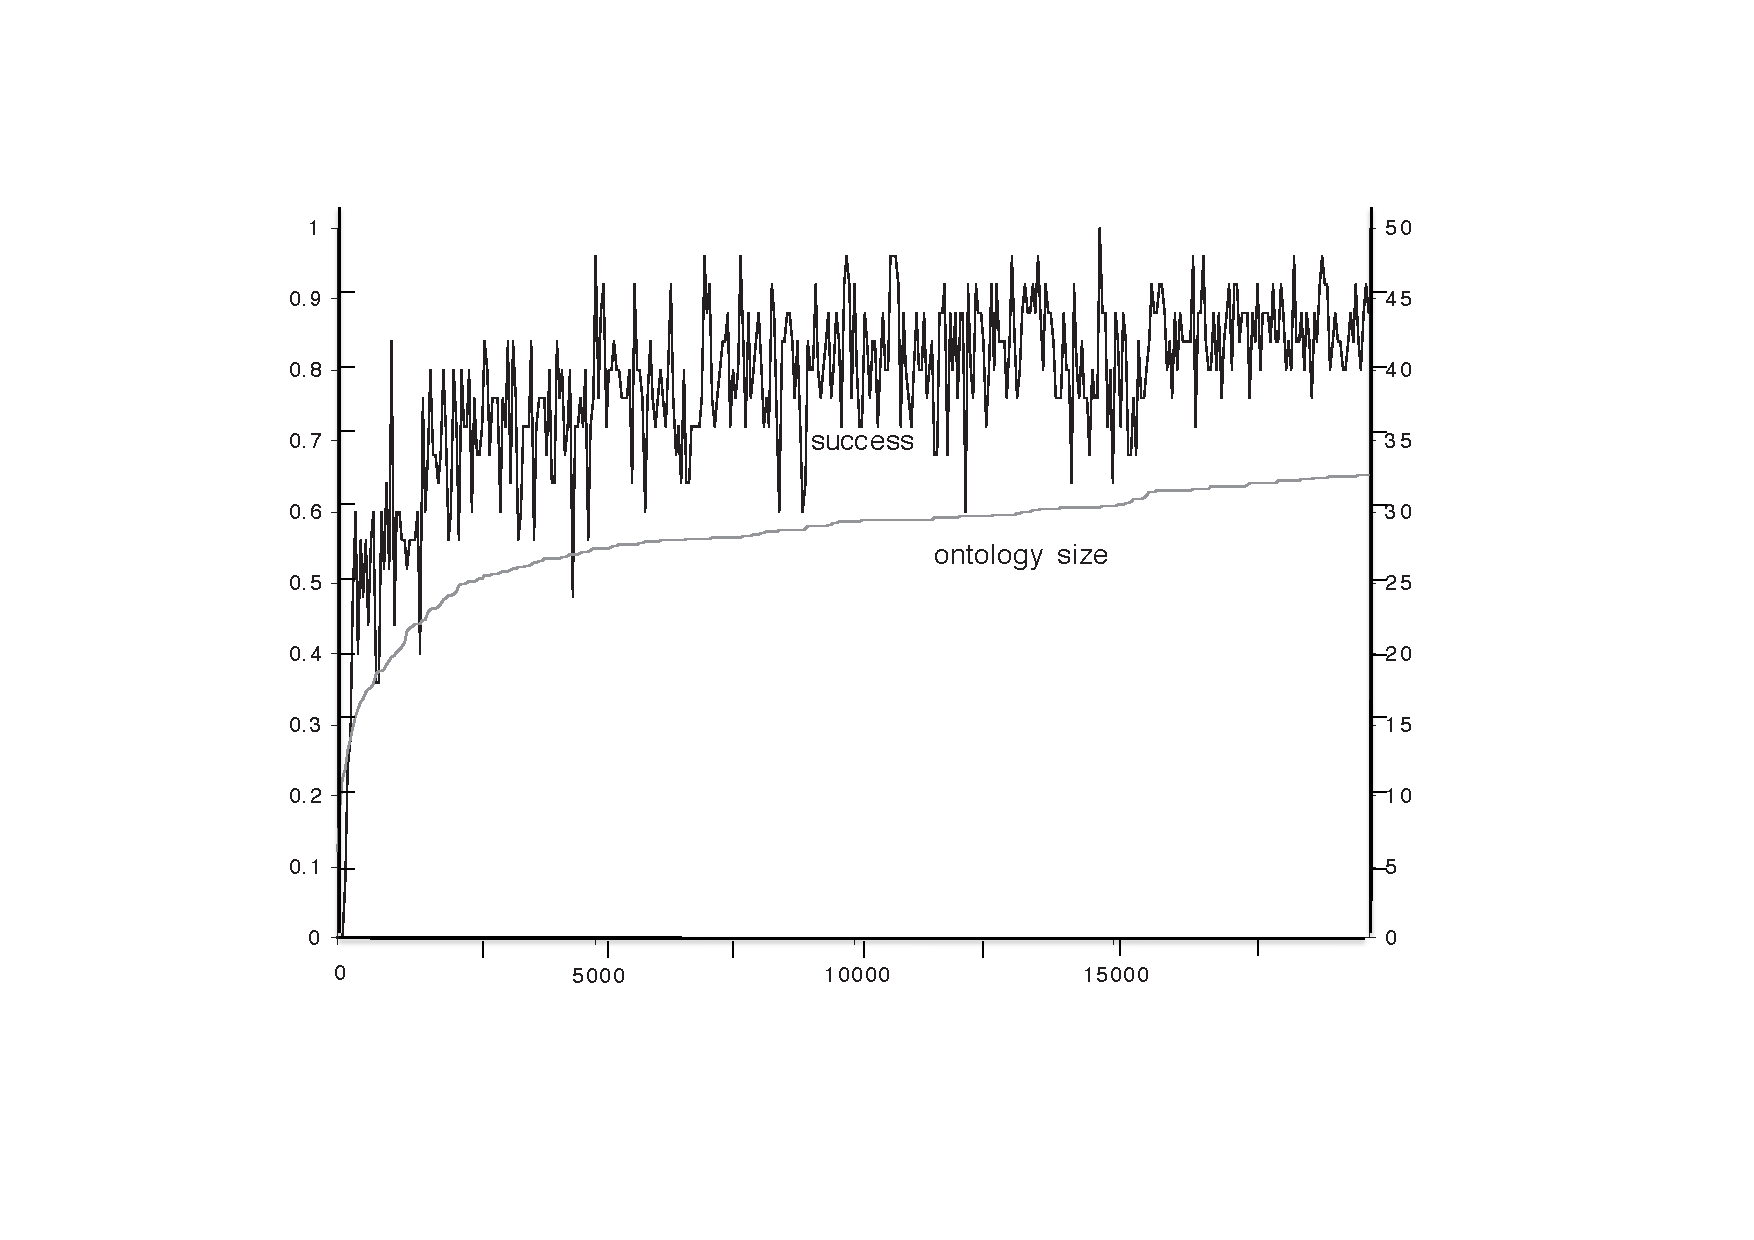
\includegraphics[width=\textwidth]{chap6/figs/agnt10.pdf}}
\caption{\label{agnt10}Communicative 
success (left y-axis) and average ontology size 
(right y-axis) for a series of 20,000 
language games played by ten agents.} 
\end{figure}

It is instructive to examine in detail the lexicon 
that has emerged after this series, where every agent
has on average played about 2000 games. The table shown in \tabref{tab:after2000} 
shows word-meaning pairs whose 
frequency is larger than 0.8. 


\begin{table}
\begin{center}
\begin{tabular}{ l  l  l  l  l }
\lsptoprule
{\itshape Word}&{\itshape Meaning}& {\itshape Translation} & {\itshape Frequency} \\ \midrule
larubo & [HPOS 0.0–0.5] & left & 1.00 \\ 
tituroxu & [HPOS 0.5–1.0] & right & 1.00 \\ 
fumetese & [VPOS 0.0–0.5] & top & 1.00 \\ 
tokadapa & [VPOS 0.5–1.0] & bottom & 1.00 \\ 
povomovi & [WIDTH 0.0–0.5] & thin & 1.00 \\ 
kilokawe & [WIDTH 0.5–1.0] & wide & 1.00 \\ 
legoka & [HEIGHT 0.0–0.5] & short & 0.94\\  
vuwusugu & [GREY 0.0–0.5] & light & 1.00 \\ 
kewenoku & [GREY 0.5–1.0] & dark & 1.00 \\ 
\lspbottomrule
\end{tabular}
\caption{\label{tab:after2000}Group lexicon after 2000 games.}
\end{center}
\end{table}

We see that for all the sensory channels, solid words
exist for the top level categories. There is however
one exception: there are no words in this group for AREA
nor for [HEIGHT 0.5–1.0]. We do find these words, and 
words for more refined notions as well, in the 
batch of word-meaning pairs whose scores are between 0.5 and 0.8, shown 
in \tabref{tab:freq}. 


\begin{table}
\begin{center}
\begin{tabular}{ l  l  l  l }
\lsptoprule
{\itshape Word}&{\itshape Meaning}& {\itshape Translation} & {\itshape Frequency} \\ \midrule
nifavipa & (HPOS 0.0–0.25) & very left & 0.55 \\ 
nodanova & (VPOS 0.0–0.25) & very top & 0.58  \\ 
texiraxi & (HEIGHT 0.5–1.0) & tall & 0.69  \\ 
poxalu & (HEIGHT 0.0–0.25) & very short & 0.70  \\ 
fovibilo & (HEIGHT 0.25–0.5) & medium short & 0.61  \\ 
wixizode & (AREA 0.5–1.0) & large & 0.78  \\ 
tebuwona & (GREY 0.75–1.0) & very dark & 0.76  \\ 
mogevo & (GREY 0.25–0.5) & medium light & 0.60  \\ 
toduwe & (GREY 0.0–0.25) & very light & 0.65  \\ 
\lspbottomrule
\end{tabular}
\caption{\label{tab:freq}Table of word meaning pairs and their average scores.}
\end{center}
\end{table}
Although most of these words are on their way towards
total coherence, because the competition has already 
been damped completely, this is less the case for 
the AREA/HEIGHT words. Closer inspection reveals that 
there are two words competing for expressing
AREA and HEIGHT: `texiraxi' and `wixizode'
(\figref{triangle7}). Both words have both meanings
but there is a strong divergence of opinion in the 
population. Some prefer the AREA meaning, others prefer
the HEIGHT meaning. This can be seen from the scores of 
the different meanings.


\begin{figure}[htbp]
  \centerline{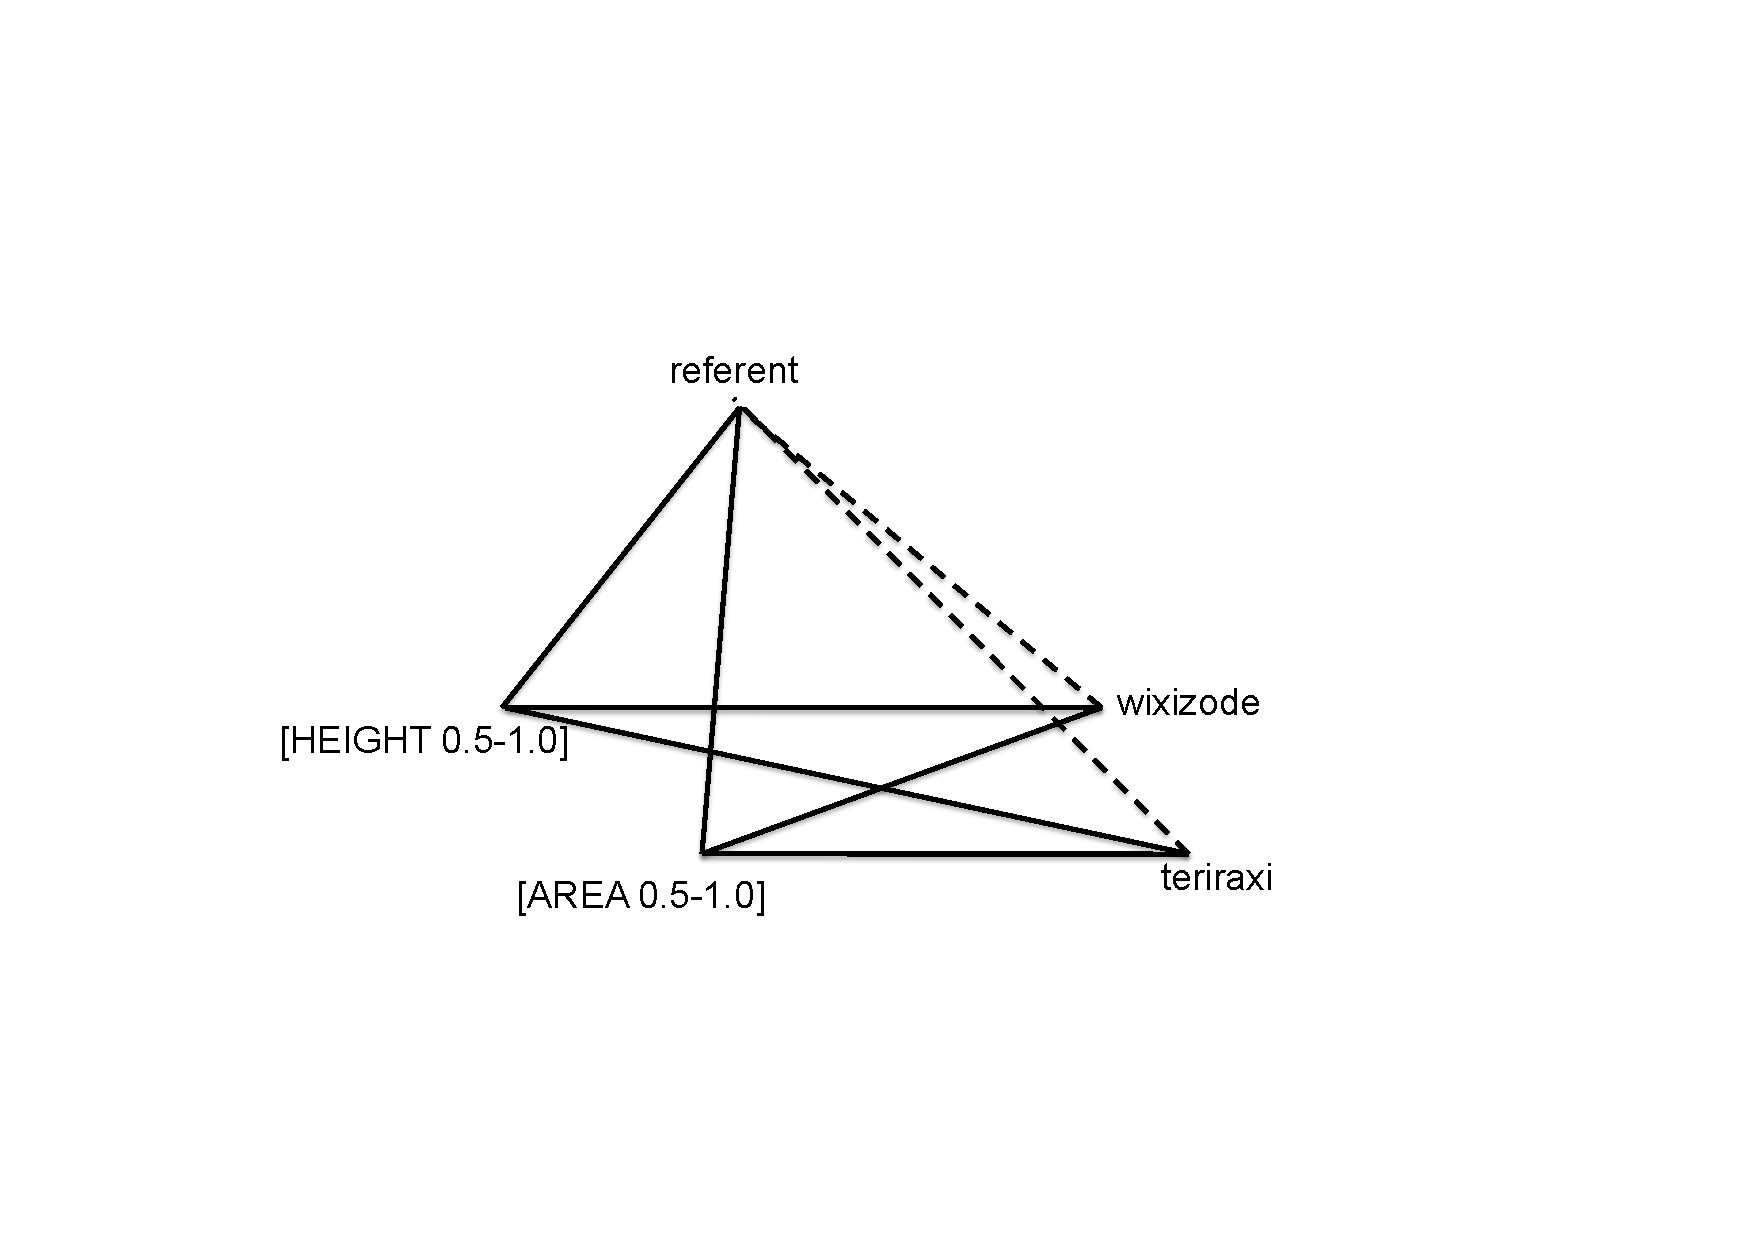
\includegraphics[width=.60\textwidth]{chap6/figs/triangle7.pdf}}
\caption{\label{triangle7}Two different words have the 
same two meanings and have difficulty disambiguating because
they are often both equally distinctive in a given situation.}
\end{figure}
For the word texiraxi, the scores of the different 
agents for the AREA and HEIGHT categories is as in \tabref{tab:texiraxi}. 


\begin{table}
\begin{center}
\begin{tabular}{ l  l  l  l  l }
\lsptoprule
{\itshape Agent} & 
\multicolumn{2}{c }{\itshape Scores `texiraxi'} &
\multicolumn{2}{c }{\itshape Scores `wixizode'}\\ 
 & HEIGHT & AREA  & HEIGHT & AREA \\ \midrule
a1 & 0.00 & 0.9 & 0.6 & 0.4\\  
a2 & 0.0 & 1.0  & 1.0 & 0.0\\ 
a3 & 0.90 & 0.2  & 0.0 & 1.0\\ 
a4 & 1.00 & 0.0  & 0.0 & 1.0\\ 
a5 & 1.00  &  0.0  & 0.2  &  0.6\\ 
a6 & 1.00 & 0.0   & 0.0 & 1.0  \\ 
a7 & 1.00 & 0.0  & 1.00 & 1.0\\ 
a8 & 1.00 & 0.0  & 1.00 & 1.0 \\ 
a9 & 1.00 & 0.0 & 1.00 & 1.0 \\ 
a10 & 0.0 & 1.0  & 0.0 & 0.8 \\ 
\lspbottomrule
\end{tabular}
\caption{\label{tab:texiraxi}Scores for area and height categories.}
\end{center}
\end{table}
A game where the two meanings are compatible is shown below: 
\begin{verbatim}
Game 10008
  a2 is the speaker. a4 is the hearer. 
  a2 segments the context into 2 objects: 
       circle-0 square-1
  a2 chooses square-1 as the topic 
  a2 considers as salient AREA WIDTH HEIGHT
  a2 categorises the topic as 
{}[HEIGHT 0.5–1.0] [HEIGHT 0.75–1.0] 
{}[WIDTH 0.5–1.0] [WIDTH 0.75–1.0] 
{}[AREA 0.5–1.0] [AREA 0.75–1.0] 
{}[HEIGHT 0.5–1.0] [HEIGHT 0.75–1.0] 
  a2 has the words
      wixizode for [HEIGHT 0.5–1.0] (1.0)
      kilokawe for [WIDTH 0.5–1.0] (1.0)
      texiraxi for [AREA 0.5–1.0] (1.0)
      powugeme for [HEIGHT 0.5–1.0] (0.8)
      wetami for [HEIGHT 0.75–1.0] (0.5)
      wofetizo for [WIDTH 0.5–1.0] (0.4)
      kufule for [HEIGHT 0.75–1.0] (0.1)
      lisexese for [HEIGHT 0.75–1.0] (0.1)
  a2 says: `wixizode'
  a7 interprets `wixizode' as
{}[AREA 0.5–1.0] (1.0)
{}[WIDTH 0.0–0.5] (0.0)
{}[HEIGHT 0.5–1.0] (0.0)
  a7 identifies square-1
  a2 signals OK
\end{verbatim}
Note the abundance of choices for the speaker. He finally 
picks `wixizode'. The hearer interprets this using AREA
and the game succeeds. A partial overview of the different 
choices and subsequent updating is given in \figref{incr-decr2}. 
The speaker decreases the score of `powugeme' which is 
also competing for expressing [HEIGHT 0.5–1.0]. 
The hearer on the other hand damps the alternative meanings 
of `wixizode', which includes
the meaning [HEIGHT 0.5–1.0] used by the speaker. 

This example shows that there will be a divergence of 
opinion among the agents if the environment does not 
provide enough 
disambiguating cases. It is still possible of course that 
the semantic incoherence will disappear from the lexicon, 
but it is understandable that agents have difficulty 
in this domain to disentangle the meanings of words for 
tall and large. French has one word `grand' encapsulating
both of these categories.

Here are the words in the lexicon with still lower 
frequencies in the population (between 0.2 and 0.5). We see
more clearly several synonyms in heavy competition, for example 
`kodawika' and `togixa' for [GRAY 0.5.0.75], or 
`vavuvosi' and `radude' for [WIDTH 0.75–1.0]. See \tabref{tab:comp}. 


\begin{table}
\begin{center}
\begin{tabular}{ l  l  l }
\lsptoprule
{\itshape Word}&{\itshape Meaning} & {\itshape Frequency} \\ \midrule
lovifo & [HPOS 0.5–0.75] & 0.21 \\ 
petenuga & [HPOS 0.5–0.75] & 0.25 \\ 
gafizuru & [WIDTH 0.25–0.5] & 0.24 \\ 
vavuvosi & [WIDTH 0.5–0.75] & 0.27 \\ 
radude & [WIDTH 0.5–0.75] & 0.30 \\ 
wofetizo & [WIDTH 0.75–1.0] & 0.42 \\ 
wetami & [HEIGHT 0.75–1.0] & 0.40 \\ 
donadewe & [HEIGHT 0.5–0.75] & 0.41 \\ 
turede & [AREA 0.0–0.25] & 0.26 \\ 
likiwewe & [AREA 0.0–0.5] & 0.27 \\ 
savifo & [AREA 0.25–0.5] & 0.21 \\ 
rapoguwe & [AREA 0.5–0.75] & 0.22 \\ 
texiraxi & [AREA 0.5–1.0] & 0.31 \\ 
kodawika & [GREY 0.5–0.75] & 0.23 \\ 
togixa & [GREY 0.5–0.75] & 0.45 \\ 
\lspbottomrule
\end{tabular}
\caption{\label{tab:comp}Lexicon with lower frequencies.}
\end{center}
\end{table}

So all the mechanisms proposed earlier 
do what they are supposed to do, even when we 
scale up the population. The Discrimination 
Game generates the repertoire of distinctions 
necessary in this domain, the Naming Game generates
the shared repertoire of form-meaning pairs. The 
coupling between the two based on feedback from 
the environment causes a convergence even if the
agents do not have any direct knowledge about 
which meanings are used by the others. 

\subsection{Lexicon acquisition by new agents}

We finally scale up on the same dimension but 
now towards an open population. The following 
simulation examines what happens when a new agent 
enters into the population. The agent has no 
prior ontology nor any knowledge of the existing
lexicon in the group and no additional components
or processes are added, compared to the agents
in the simulation so far. Introducing a new 
agent tests in how far the cognitive architecture
put in place enables a new agent to acquire a 
lexicon that already exists. 

The first words learned (after about a dozen 
games by the agent) are shown in \tabref{tab:first}. 


\begin{table}
\begin{center}
\begin{tabular}{ l  l  l  l  l }
\lsptoprule
{\itshape Word} & {\itshape Meaning} & {\itshape Score} \\ \midrule
larubo  & [HPOS 0.0–0.5] & 0.30 \\ 
sakezomo &  [HPOS 0.0–0.5] & 0.00 \\ 
tituroxu &  [HPOS 0.5–1.0] & 0.50 \\ 
tokadapa & [VPOS 0.5–1.0] & 0.20 \\ 
legoka   & [HEIGHT 0.0–0.5] & 0.30 \\ 
kuvodogi  & [WIDTH 0.0–0.5] & 0.00 \\ 
gafizuru &  [WIDTH 0.25–0.5] & 0.10  \\ 
nopofi  & [WIDTH 0.5–1.0] & 0.00 \\ 
\lspbottomrule
\end{tabular}
\caption{\label{tab:first}First words after about a dozen games.}
\end{center}
\end{table}

As expected, the new 
agent sometimes creates new words (this is the case 
for `sakezomo' and `nopofi'). But these words are 
very short-lived. The new agent has already picked up 
`larubo' which is the word in use expressing the 
meaning of `sakezomo'. `larubo' has already a higher 
score so `sakezomo' will definitely disappear. 

The most widespread words in the lexicon 
such as `tituroxu' or `legoka' are the ones that 
are most likely to be picked up because the chance
that they will be heard is higher. This suggests
that the entry of new agents in the population does
not destabilise the lexicon but on the contrary 
it makes it more coherent \footnote{The importance of a flux in the agent population for
streamlining a language has been stressed by Simon Kirby, who 
has applied this principle in a remarkable simulation 
concerning the origins of hierarchical structure, \cite{Kirby:1999}.}

For example, the new agent
has solidly associated the word `texiraxi' with 
{}[HEIGHT 0.5–1.0] and `wixizode' with [AREA 0.5–1.0]
as the majority of the population. Thus resolving the 
incoherence shown in \figref{triangle7}. 

Notice also that the new agent first acquires words 
for the more abstract categories. This is the case 
because (1) the discrimination trees are still developing
and so more specific categories are not yet available, 
and (2) even if more specific categories are available, 
agents do not try to be more specific than needed in 
the game. 

\tabref{tab:newagents} is the set of words of the new agent
with scores above 0.4 after 
500 total games (which means more or less 100 games 
in which the new agent was involved). 


\begin{table}
\begin{center}
\begin{tabular}{ l  l  l }
\lsptoprule
{\itshape Word} & {\itshape Meaning} & {\itshape Score} \\ \midrule
texiraxi &  [HEIGHT 0.5–1.0] & 0.80 \\ 
lepowaxu &  [HEIGHT 0.25–0.5] & 0.50 \\ 
kewenoku &  [GREY 0.5–1.0] & 0.80 \\ 
wixizode & [AREA 0.5–1.0] & 1.00 \\ 
vuwusugu & [GREY 0.0–0.5] & 0.50 \\ 
tokadapa &  [VPOS 0.5–1.0] & 1.00 \\ 
tituroxu &  [HPOS 0.5–1.0] & 1.00 \\ 
legoka   &  [HEIGHT 0.0–0.5] & 1.00 \\ 
larubo   &  [HPOS 0.0–0.5] & 1.00 \\ 
fumetese &  [WIDTH 0.0–0.5] & 0.40 \\ 
\lspbottomrule
\end{tabular}
\caption{\label{tab:newagents}Score of new agent after 500 games.}
\end{center}
\end{table}
The agent clearly picks up the lexicon circulating
in the population and generally associates the 
same meanings to the words (compare with the 
lexicons given earlier for the total population). 
Occasionally there are still incoherences. For example, 
`fumetese' has been associated with [WIDTH 0.0–0.5] 
whereas the rest of the population uses this word
for a distinction on the VPOS-channel. The meaning
of this word will later shift as the agent encounters
disambiguating cases. We can conclude that the 
guessing game shows not only how a population may 
emerge a lexicon from scratch but also how new 
agents entering the group may acquire the existing 
lexicon.  

\section{Conclusions}

This chapter has coupled the Discrimination Game and 
the Naming Game, so that agents now can play language
games without getting explicit feedback about meanings. 
As in the case of humans, feedback only comes through 
the non-verbal outcome of a game. 
This may generate semantic confusion
because usually more than one conceptualisation is 
possible to distinguish a topic from the other objects
in the context. However we have seen that despite
this complication agents still manage to build up 
an ontology and a lexicon which is effective for 
communicating in their environment. 

Although this chapter took away the assumption of 
direct meaning feedback, it still made a number of 
simplifying assumptions with respect to real world
physical agents, in particular it assumed that 
the perception of the scene was identical for
the speaker and the hearer. The next chapter takes away 
this assumption and thus sets the final step to test 
whether a perceptually grounded lexicon may 
emerge in a population of {\itshape embodied} distributed 
autonomous agents. 

